\documentclass[a4paper]{article}
\usepackage[colorlinks,linkcolor=black,urlcolor=black]{hyperref}
\usepackage{float}
\usepackage{mhchem}
\usepackage{pdfpages}
\usepackage{enumerate}
\usepackage{amsmath}
\usepackage{amssymb}
\usepackage{graphicx}
\usepackage{subfigure}
\usepackage{wrapfig}
\usepackage{geometry}
\usepackage{indentfirst}
\usepackage{array}
\usepackage{multirow} 
\setlength{\parindent}{2em}
\usepackage[greek,english]{babel} 
\geometry{left=2cm,right=2cm,top=1.5cm,bottom=1.5cm}

\begin{document}

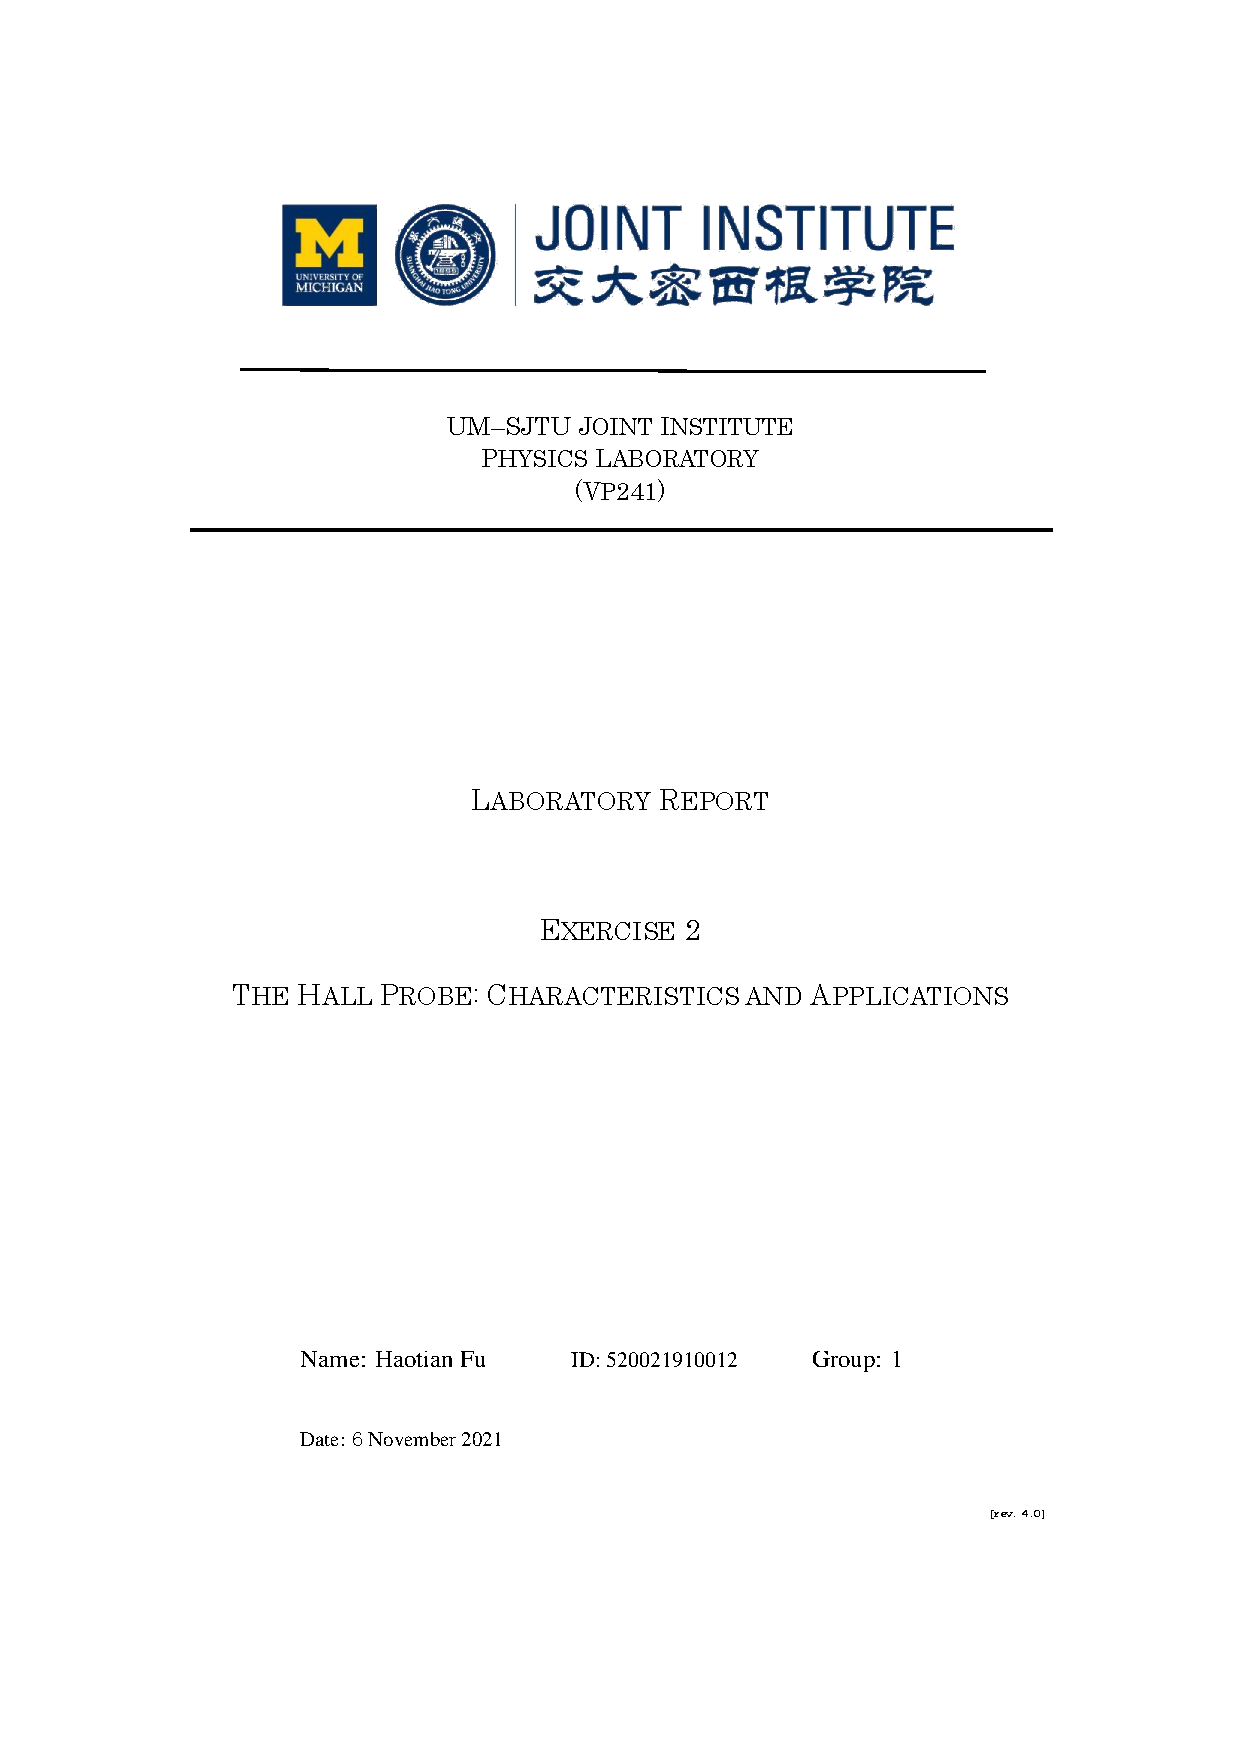
\includepdf{lab2_cover.pdf}

\newpage
\tableofcontents
\setcounter{page}{1}

\newpage
\listoffigures
\listoftables

\newpage
\section{Introduction}
The objective of this exercise is basically to use a Hall probe to verify the Hall effect and apply it to measure magnetic field.

\subsection{Basic Concepts}
\begin{itemize}
	\item \textbf{Hall Effect:}$^{[1]}$ The Hall effect is the production of a voltage difference (the Hall voltage) across an electrical conductor that is transverse to an
	      electric current in the conductor and to an applied magnetic field perpendicular to the current. It was discovered by Edwin Hall in 1879.
	\item \textbf{Lorentz Force:}$^{[2]}$ Lorentz force (or electromagnetic force) is the combination of electric and magnetic force on a point charge due to electromagnetic
	      fields.
	\item \textbf{Integrated Hall Probe:}$^{[3]}$ A device that arranges the Hall probe and the electric circuits together.
\end{itemize}

\subsection{Hall Effect}
\subsubsection{The Principle of the Hall Effect}
\par For a conducting sheet (made of a metal or a semiconductor) placed in a magnetic field, assume the plane of the sheet is vertical to the direction of the magnetic field
\textbf{B} and the electric current $I$ passes through the sheet in the direction of shown in  Fig.(\ref{fig::the principle}). Hence an electric potential difference
between  the sides $a$ and $b$ of the sheet is generated. The corresponding electric field is perpendicular to both the direction of the current and the direction of the
magnetic field. This effect is known as \textbf{the Hall effect}, ang we name the electric potential difference as \textbf{the Hall voltage} $U_H$.
\begin{figure}[!htbp]
	\centering
	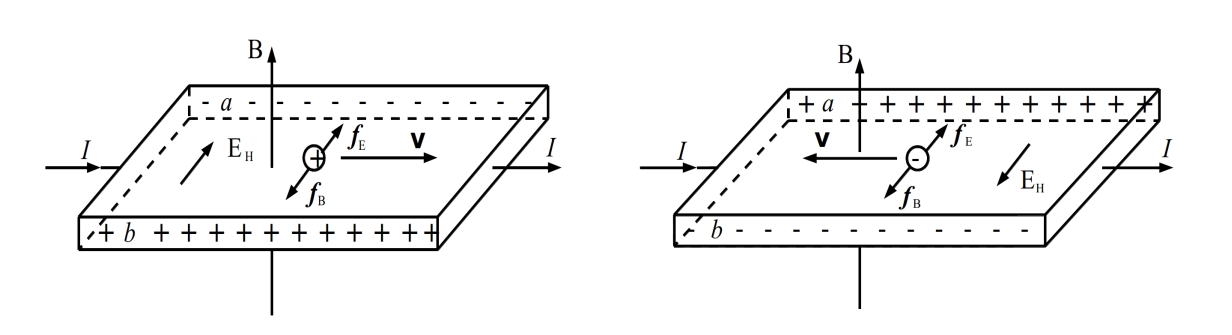
\includegraphics[width=0.8\textwidth]{the principle.png}
	\caption{The principle of the Hall effect}
	\label{fig::the principle}
\end{figure}
\subsubsection{Lorentz Force}
\par In a microscopical point of view, the Hall effect is caused by \textbf{Lorentz force}. The Lorentz force $ F_B $ leads to the deflection of the moving charges,
and their accumulation on one side of the sheet, which in turn increases the magnitude of the transverse electric field $ E_H $. Due to this field, there is an electric
force $ F_E $ acting upon the charges, and since $ F_B $ and $ F_E $ act in opposite directions, a balance is eventually reached and $ U_H $ stabilizes.
\begin{figure}[!htbp]
	\centering
	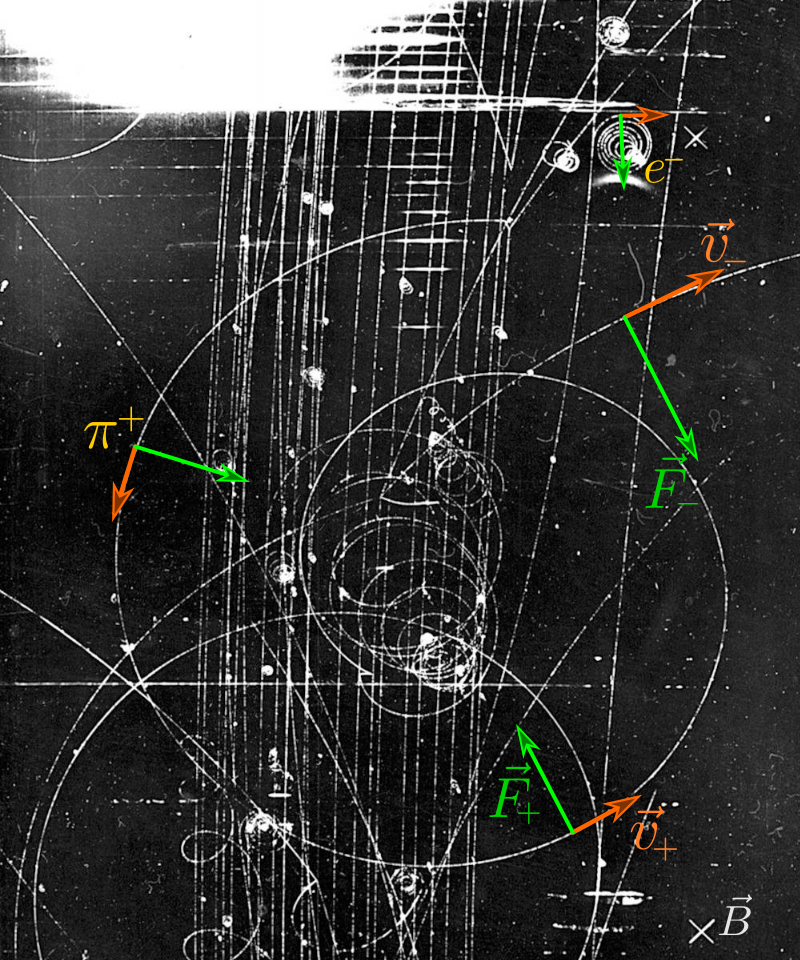
\includegraphics[width=0.25\textwidth]{Lorentz_force_on_charged_particles_in_bubble_chamber.png}
	\caption{Lorentz force acting on fast-moving charged particles in a bubble chamber$^{[2]}$}
\end{figure}
\subsubsection{Formula}
\par When the external magnetic field is not too strong, the Hall voltage is proportional to both the current and the magnitude of the magnetic field, and inversely
proportional to the thickness of the sheet $d$
\begin{equation}
	U_H=R_H\dfrac{IB}{d}=KIB
\end{equation}
where $ R_H $ is the so-called Hall coefficient and $ K=R_H/d=K_H/I $, where $ K_H $ is the so-called sensitivity of the Hall element.

\subsection{Integrated Hall Probe}
\subsubsection{Introduction}
\par Although the magnitude of the magnetic field can be found by measuring the Hall voltage with a Hall probe when the sensitivity $K_H$ and the current $I$ are fixed,
the Hall voltage is usually very small, it should be amplified before the measurement.
\par Silicon can be used to design both the Hall probe and the integrated circuits, so it is convenient to arrange the Hall probe and the electric circuits into a single
device. Such a device is called an \textbf{integrated Hall probe}.
\subsubsection{Example}
The integrated Hall probe SS495A consists of a Hall sensor, an amplifier, and a voltage compensator (Fig.(2)). The output voltage U can be read ignoring the residual
voltage. The working voltage $ U_S = 5 V $, and the output voltage $ U_0 $ is approximately $ 2.5 V $ when the magnetic field is zero. The relation between the output
voltage U and the magnitude of the magnetic field is
\begin{equation}
	B=\dfrac{U-U_0}{K_H}
	\label{eq::magnetic field}
\end{equation}
\begin{figure}[!htbp]
	\centering
	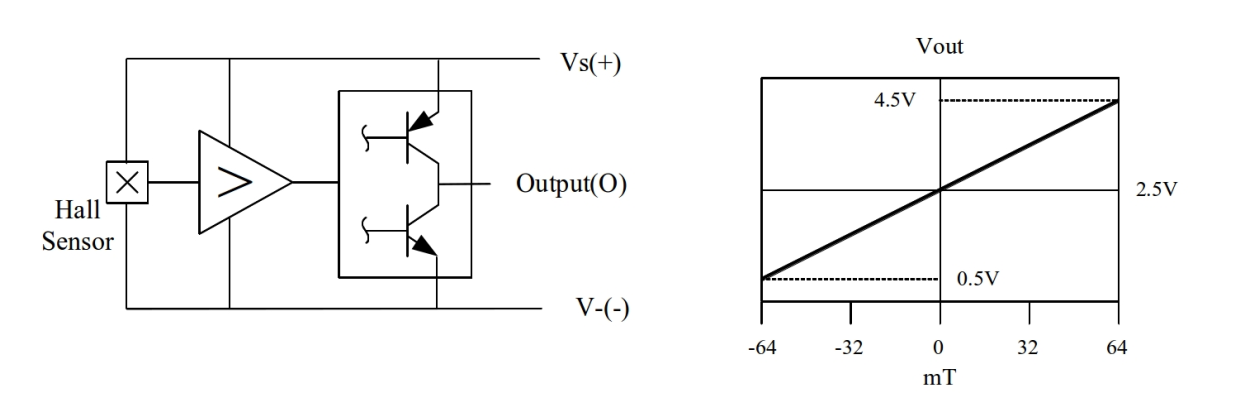
\includegraphics[width=0.8\textwidth]{integrated Hall probe.png}
	\caption{The integrated Hall probe SS495A (left). The relation between the output voltage U and the magnitude of the magnetic field B (right).}
\end{figure}

\subsection{Magnetic Field Distribution Inside a Solenoid}
Solenoid is a typical electromagnetic element. In this exercise we explore the magnetic field distribution of it with the Hall probe. The theoretical value of magnetic
field distribution on the axis of a single layer solenoid can be calculated from the following formula.
\begin{equation}
	B(x) = \mu_0\frac{N}{L}I_\text{M}\left(\frac{L+2x}{2[D^2+(L+2x)^2]^{\frac{1}{2}}}+\frac{L-2x}{2[D^2+(L-2x)^2]^{\frac{1}{2}}}\right) = C(x)I_\text{M}
	\label{eq::Bx}
\end{equation}
where $N$ is the number of turns of the solenoid, $L$ is its length, $I_\text{M}$ is the current through the solenoid wire, and D is the solenoid’s diameter. The
magnetic permeability of vacuum is $\mu_0 = 4\pi \times 10^{-7} \text{H}/\text{m}.$
\par The solenoid used in this exercise has ten layers, and the magnetic field $B(x)$ for each layer can be calculated using Eq. (\ref{eq::Bx}). Then the net magnetic
on the axis of the solenoid can be found by adding contributions due to all layers. The theoretical value of the magnetic field inside the solenoid with $I_\text{M}$ =
0.1 A is given in Table \ref{table::theoretical value}.

\begin{table}[!htbp]
	\centering
	\begin{tabular}{cc||cc}
		\hline
		$x$ [cm]  & $B$ [mT] & $x$ [cm]   & $B$ [mT] \\
		\hline
		$\pm$ 0.0 & 1.4366   & $\pm$ 8.0  & 1.4057   \\
		$\pm$ 1.0 & 1.4363   & $\pm$ 9.0  & 1.3856   \\
		$\pm$ 2.0 & 1.4356   & $\pm$ 10.0 & 1.3478   \\
		$\pm$ 3.0 & 1.4343   & $\pm$ 11.0 & 1.2685   \\
		$\pm$ 4.0 & 1.4323   & $\pm$ 11.5 & 1.1963   \\
		$\pm$ 5.0 & 1.4292   & $\pm$ 12.0 & 1.0863   \\
		$\pm$ 6.0 & 1.4245   & $\pm$ 12.5 & 0.9261   \\
		$\pm$ 7.0 & 1.4173   & $\pm$ 13.0 & 0.7233   \\
		\hline
	\end{tabular}
	\caption{Theoretical value of the magnetic field inside the solenoid.}
	\label{table::theoretical value}
\end{table}

\section{Apparatus and Measurement Procedure}

\subsection{Apparatus}
The experimental setup (Fig.(\ref{fig::Apparatus})) consists of an integrated Hall probe SS495A (Fig. (\ref{fig::SS495A})) with $K_\text{H}$ = 31.25 $\pm$ 1.25 V/T (at the
working voltage 5$\,$V) or $K_\text{H} = 3.125\pm0.125$ mV/G, a solenoid, a power supply, a voltmeter, a DC voltage divider, and a set of connecting wires.
\begin{figure}[!htbp]
	\centering
	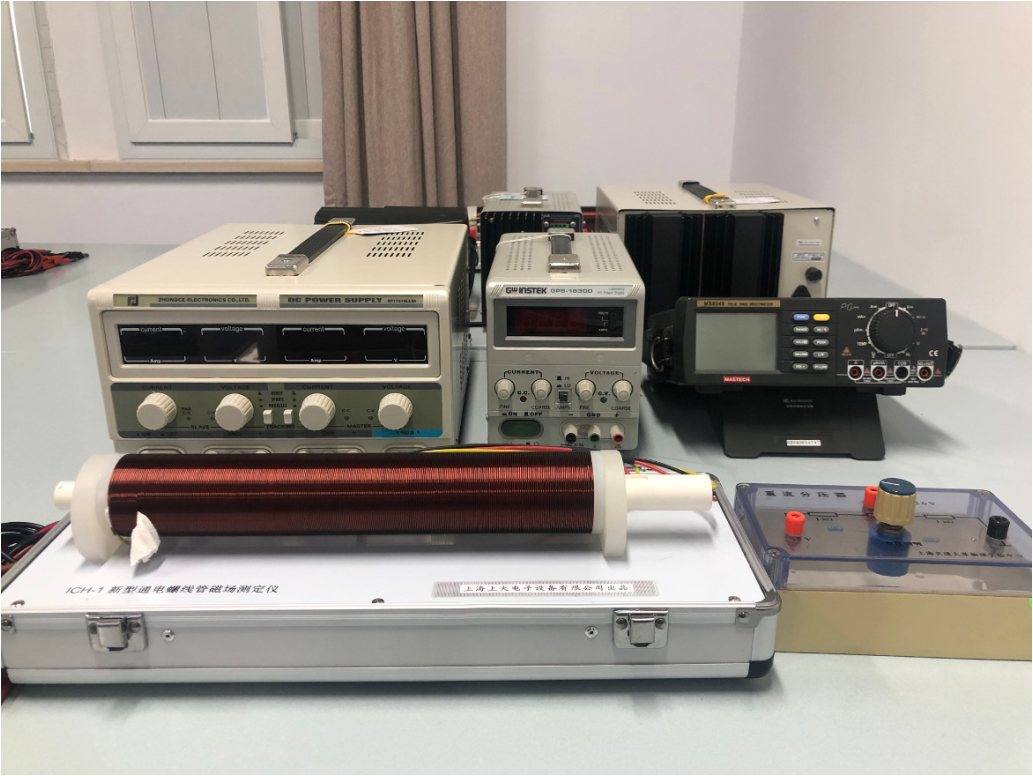
\includegraphics[width=0.7\textwidth]{Apparatus.png}
	\caption{Apparatus}
	\label{fig::Apparatus}
\end{figure}
\begin{figure}[!htbp]
	\centering
	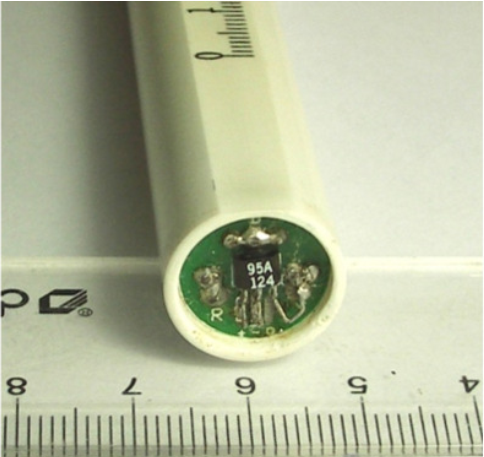
\includegraphics[width=0.4\textwidth]{SS495A.png}
	\caption{Integrated Hall probe SS495A}
	\label{fig::SS495A}
\end{figure}\\
The precisions of the devices are shown in Table \ref{table::Precision}.
\begin{table}[htbp]
	\centering
	\begin{tabular}{ccc}
		\hline
		Instrument      & Measured quantities       & Uncertainties                         \\
		\hline
		Voltage source  & Working voltage $U_{s}$   & $0.5\%\,$V                            \\
		Multimeter      & Output voltage $U_{0}, U$ & $0.05\% + 6\times 10^{-3}/10^{-4}\,$V \\
		Current source  & Current $I_{0}, I_{M}$    & $2\%\,$mA                             \\
		Graduated ruler & Distance                  & $0.05\,$cm                            \\
		\hline
	\end{tabular}
	\caption{Information of measurement instruments.}
	\label{table::Precision}
\end{table}

\subsection{Measurement Procedure}

\subsubsection{Relation Between Sensitivity $ K_H $ and Working Voltage $ U_S $}
In this part, we explored the relation between sensitivity $K_{H}$ and working voltage $U_{S}$ by applying Eq.(\ref{eq::magnetic field}) and measuring the corresponding
quantities.
\begin{enumerate}
	\item Place the integrated Hall probe at the center of the solenoid. Set the working voltage at 5 V and measure the output voltage $ U_0 (I_M = 0) $ and
	      $ U (I_M = 250 mA) $. Take the theoretical value of $ B(x = 0) $ from Table 1 and calculate the sensitivity of the probe $ K_H $ by using Eq. (2).
	\item Measure $ K_H $ for different values of $ U_S $ (from $ 2.8 V $ to $ 10 V $). Calculate $ K_H/U_S $ and plot the curve $ K_H/U_S\ vs.\ U_S $.
\end{enumerate}
\subsubsection{Relation Between Output Voltage $ U $ and Magnetic Field $ B $}
In this part, we explored the relation between the output voltage of the Hall probe and the magnetic field in which it is positioned by adjusting the current in the
solenoid.
\begin{enumerate}
	\item With $ B=0, U_S=5 V, $ connect the $ 2.4 \sim 2.6 V $ output terminal of the DC voltage divider and the negative port of the voltmeter. Adjust the voltage
	      until $ U_0 = 0 $.
	\item Place the integrated Hall probe at the center of the solenoid and measure the output voltage $ U $ for different values of $ I_M $ ranging from 0 to
	      $ 500 mA $, with intervals of $ 50 mA $.
	\item Explain the relation between $ B(x = 0) $ and the Hall voltage $ U_H $. Pay attention to the fact that the output voltage U is the amplified signal from
	      $ U_H $. The theoretical value of $ B(x = 0) $ can be found from Table 1.
	\item Plot the curve $ U vs. B $ and find the sensitivity $ K_H $ by a linear fit (use a computer). Compare the value you obtained with the theoretical value in
	      given in the Apparatus section.
\end{enumerate}
\subsubsection{Magnetic Field Distribution Inside the Solenoid}
In this part, we explore the magnetic field distribution inside a solenoid by adjusting the position of the Probe Hall and measuring the magnetic field at different
positions.
\begin{enumerate}
	\item Measure the magnetic field distribution along the axis of the solenoid for $ I_M = 250 mA $, record the output voltage U and the corresponding position $ x $.
	      Then find $ B = B(x) $. (Use the value of $ K_H $ found in the previous part of the experiment).
	\item Use a computer to plot the theoretical and the experimental curve showing the magnetic field distribution inside the solenoid. Use dots for the data measured
	      and a solid line for the theoretical curve. The origin of the plot should be at the center of the solenoid.
\end{enumerate}


\section{Experimental Results}

\subsection{Experiment 1 - Relationship Between Sensitivity $K_H$ and Working Voltage $U_S$}
The measurement results of $U_0$ and $U$ when $U_\text{S}$ = 5.00 V are shown in Table \ref{table::initial}.

\begin{table}[H]
	\centering
	\begin{tabular}{ccc}
		\hline
		$U_\text{S} \ [\text{V}] \pm 0.5\%\ [\text{V}]$ & $U_0 (I_\text{M} = 0) \ [\text{V}] \pm (0.05\% + 6\times10^{-3} )\ [\text{V}]$ & $U (I_\text{M} = 250\,\text{mA}) \ [\text{V}] \pm (0.05\% + 6\times10^{-3}) \ [\text{V}]$ \\
		\hline
		5.00 $\pm$ 0.03                                 & 2.504 $\pm$ 0.007                                                              & 2.621 $\pm$ 0.007                                                                         \\
		\hline
	\end{tabular}
	\caption{Data for $U_0$ and $U$ with $U_S$ = 5.00 V.}
	\label{table::initial}
\end{table}

According to the data in Table \ref{table::theoretical value}, we can obtain that when $I_\text{M} = 100 \ \text{mA},$
$B(x=0,\,I_\text{M}=100\ [\text{mA}])=1.4366\times10^{-3} \ \text{T}.$
Eq. (\ref{eq::Bx}) implies that $B$ is proportional to current $I_\text{M}$, and therefore,
\begin{equation*}
	B(x=0,I_\text{M}=250\ [\text{mA}]) = \frac{250}{100} \times 1.4366\times10^{-3} = 3.59\times 10^{-3} \pm 0.07 \times 10^{-3}\ \text{T}.
\end{equation*}
According to Eq. (\ref{eq::magnetic field}), the sensitivity of the probe $K_\text{H}$ when $U_\text{S}$ = 5.00 V is then calculated as
\begin{equation*}
	K_\text{H} = \frac{U-U_0}{B(x=0,I_\text{M}=250\,[\text{mA}])} = \frac{2.621-2.504}{3.59\times 10^{-3}} = 33 \pm 3 \,[\text{V}/\text{T}].
\end{equation*}
The measurement results of $U_0$ and $U$ for different $U_\text{S}$ are shown in Table \ref{table::e1}. We calculate $K_\text{H}/U_\text{S}$ for each set of data to
explore their relation. That is, for each set of data, we calculate
\begin{equation*}
	\frac{K_\text{H}}{U_\text{S}} = \frac{U-U_0}{BU_\text{S}}.
\end{equation*}
Taking the first set of data as an example,
\begin{equation*}
	\frac{K_\text{H}}{U_\text{S}} = \frac{U-U_0}{BU_\text{S}} = \frac{1.4656-1.4004}{3.59\times 10^{-3}\times2.80} =  6.5 \pm 0.2 \,[\text{T}^{-1}].
\end{equation*}
The measurement results and the results of calculation of $K_\text{H}/U_\text{S}$ for each set of data are presented together in Table \ref{table::e1}.
A plot of the results $K_\text{H}/U_\text{S}$ vs. $U_\text{S}$ using Origin is shown in Fig.(\ref{fig::KHUS}).
The points in the plot indicates that the ratio of $K_{H}$ to $U_{s}$ decreases as $U_{s}$ increases.

\begin{table}[htbp]
	\centering
	\begin{tabular}{c|cccc}
		\hline
		   & $U_\text{S} \,\,[\text{V}] \pm 0.5\%\,\,[\text{V}]$ & $U_0 \,\,[\text{V}] \pm (0.05\% + 6\times10^{-3/-4}\,\,[\text{V}]$ & $U \,\,[\text{V}] \pm(0.05\% + 6\times10^{-3/-4}\,\,[\text{V}]$ & $K_\text{H}/U_\text{S} \,\,[\text{T}^{-1}]$ \\
		\hline
		1  & 2.80 $\pm$ 0.014                                    & 1.4004 $\pm$ 0.0013                                                & 1.4656 $\pm$ 0.0014                                             & 6.5 $\pm$ 0.2                               \\
		2  & 3.20 $\pm$ 0.016                                    & 1.6002 $\pm$ 0.0014                                                & 1.6760 $\pm$ 0.0015                                             & 6.6 $\pm$ 0.2                               \\
		3  & 3.60 $\pm$ 0.018                                    & 1.8022 $\pm$ 0.0015                                                & 1.8905 $\pm$ 0.0016                                             & 6.8 $\pm$ 0.2                               \\
		4  & 4.00 $\pm$ 0.020                                    & 2.002 $\pm$ 0.007                                                  & 2.097 $\pm$ 0.007                                               & 6.6 $\pm$ 0.2                               \\
		5  & 4.40 $\pm$ 0.022                                    & 2.201 $\pm$ 0.008                                                  & 2.308 $\pm$ 0.008                                               & 6.8 $\pm$ 0.5                               \\
		6  & 4.80 $\pm$ 0.024                                    & 2.405 $\pm$ 0.008                                                  & 2.518 $\pm$ 0.008                                               & 6.6 $\pm$ 0.6                               \\
		7  & 5.20 $\pm$ 0.026                                    & 2.602 $\pm$ 0.008                                                  & 2.723 $\pm$ 0.008                                               & 6.5 $\pm$ 0.6                               \\
		8  & 5.60 $\pm$ 0.028                                    & 2.800 $\pm$ 0.008                                                  & 2.933 $\pm$ 0.008                                               & 6.6 $\pm$ 0.5                               \\
		9  & 6.00 $\pm$ 0.030                                    & 2.999 $\pm$ 0.008                                                  & 3.136 $\pm$ 0.008                                               & 6.4 $\pm$ 0.5                               \\
		10 & 6.40 $\pm$ 0.032                                    & 3.198 $\pm$ 0.008                                                  & 3.343 $\pm$ 0.008                                               & 6.3 $\pm$ 0.5                               \\
		11 & 6.80 $\pm$ 0.034                                    & 3.394 $\pm$ 0.008                                                  & 3.545 $\pm$ 0.008                                               & 6.2 $\pm$ 0.5                               \\
		12 & 7.20 $\pm$ 0.036                                    & 3.592 $\pm$ 0.008                                                  & 3.748 $\pm$ 0.008                                               & 6.0 $\pm$ 0.4                               \\
		13 & 7.60 $\pm$ 0.038                                    & 3.788 $\pm$ 0.008                                                  & 3.952 $\pm$ 0.008                                               & 6.0 $\pm$ 0.4                               \\
		14 & 8.00 $\pm$ 0.040                                    & 3.988 $\pm$ 0.008                                                  & 4.152 $\pm$ 0.008                                               & 5.7 $\pm$ 0.4                               \\
		15 & 8.40 $\pm$ 0.042                                    & 4.183 $\pm$ 0.008                                                  & 4.351 $\pm$ 0.009                                               & 5.6 $\pm$ 0.4                               \\
		16 & 8.80 $\pm$ 0.044                                    & 4.380 $\pm$ 0.009                                                  & 4.552 $\pm$ 0.009                                               & 5.4 $\pm$ 0.3                               \\
		17 & 9.20 $\pm$ 0.046                                    & 4.573 $\pm$ 0.009                                                  & 4.751 $\pm$ 0.009                                               & 5.4 $\pm$ 0.3                               \\
		18 & 10.00 $\pm$ 0.050                                   & 4.963 $\pm$ 0.009                                                  & 5.143 $\pm$ 0.009                                               & 5.0 $\pm$ 0.3                               \\
		\hline
	\end{tabular}
	\caption{Data for $U_0$, $U$ and $K_\text{H}/U_\text{S}$ for different $U_\text{S}$.}
	\label{table::e1}
\end{table}

\begin{figure}[H]
	\centering
	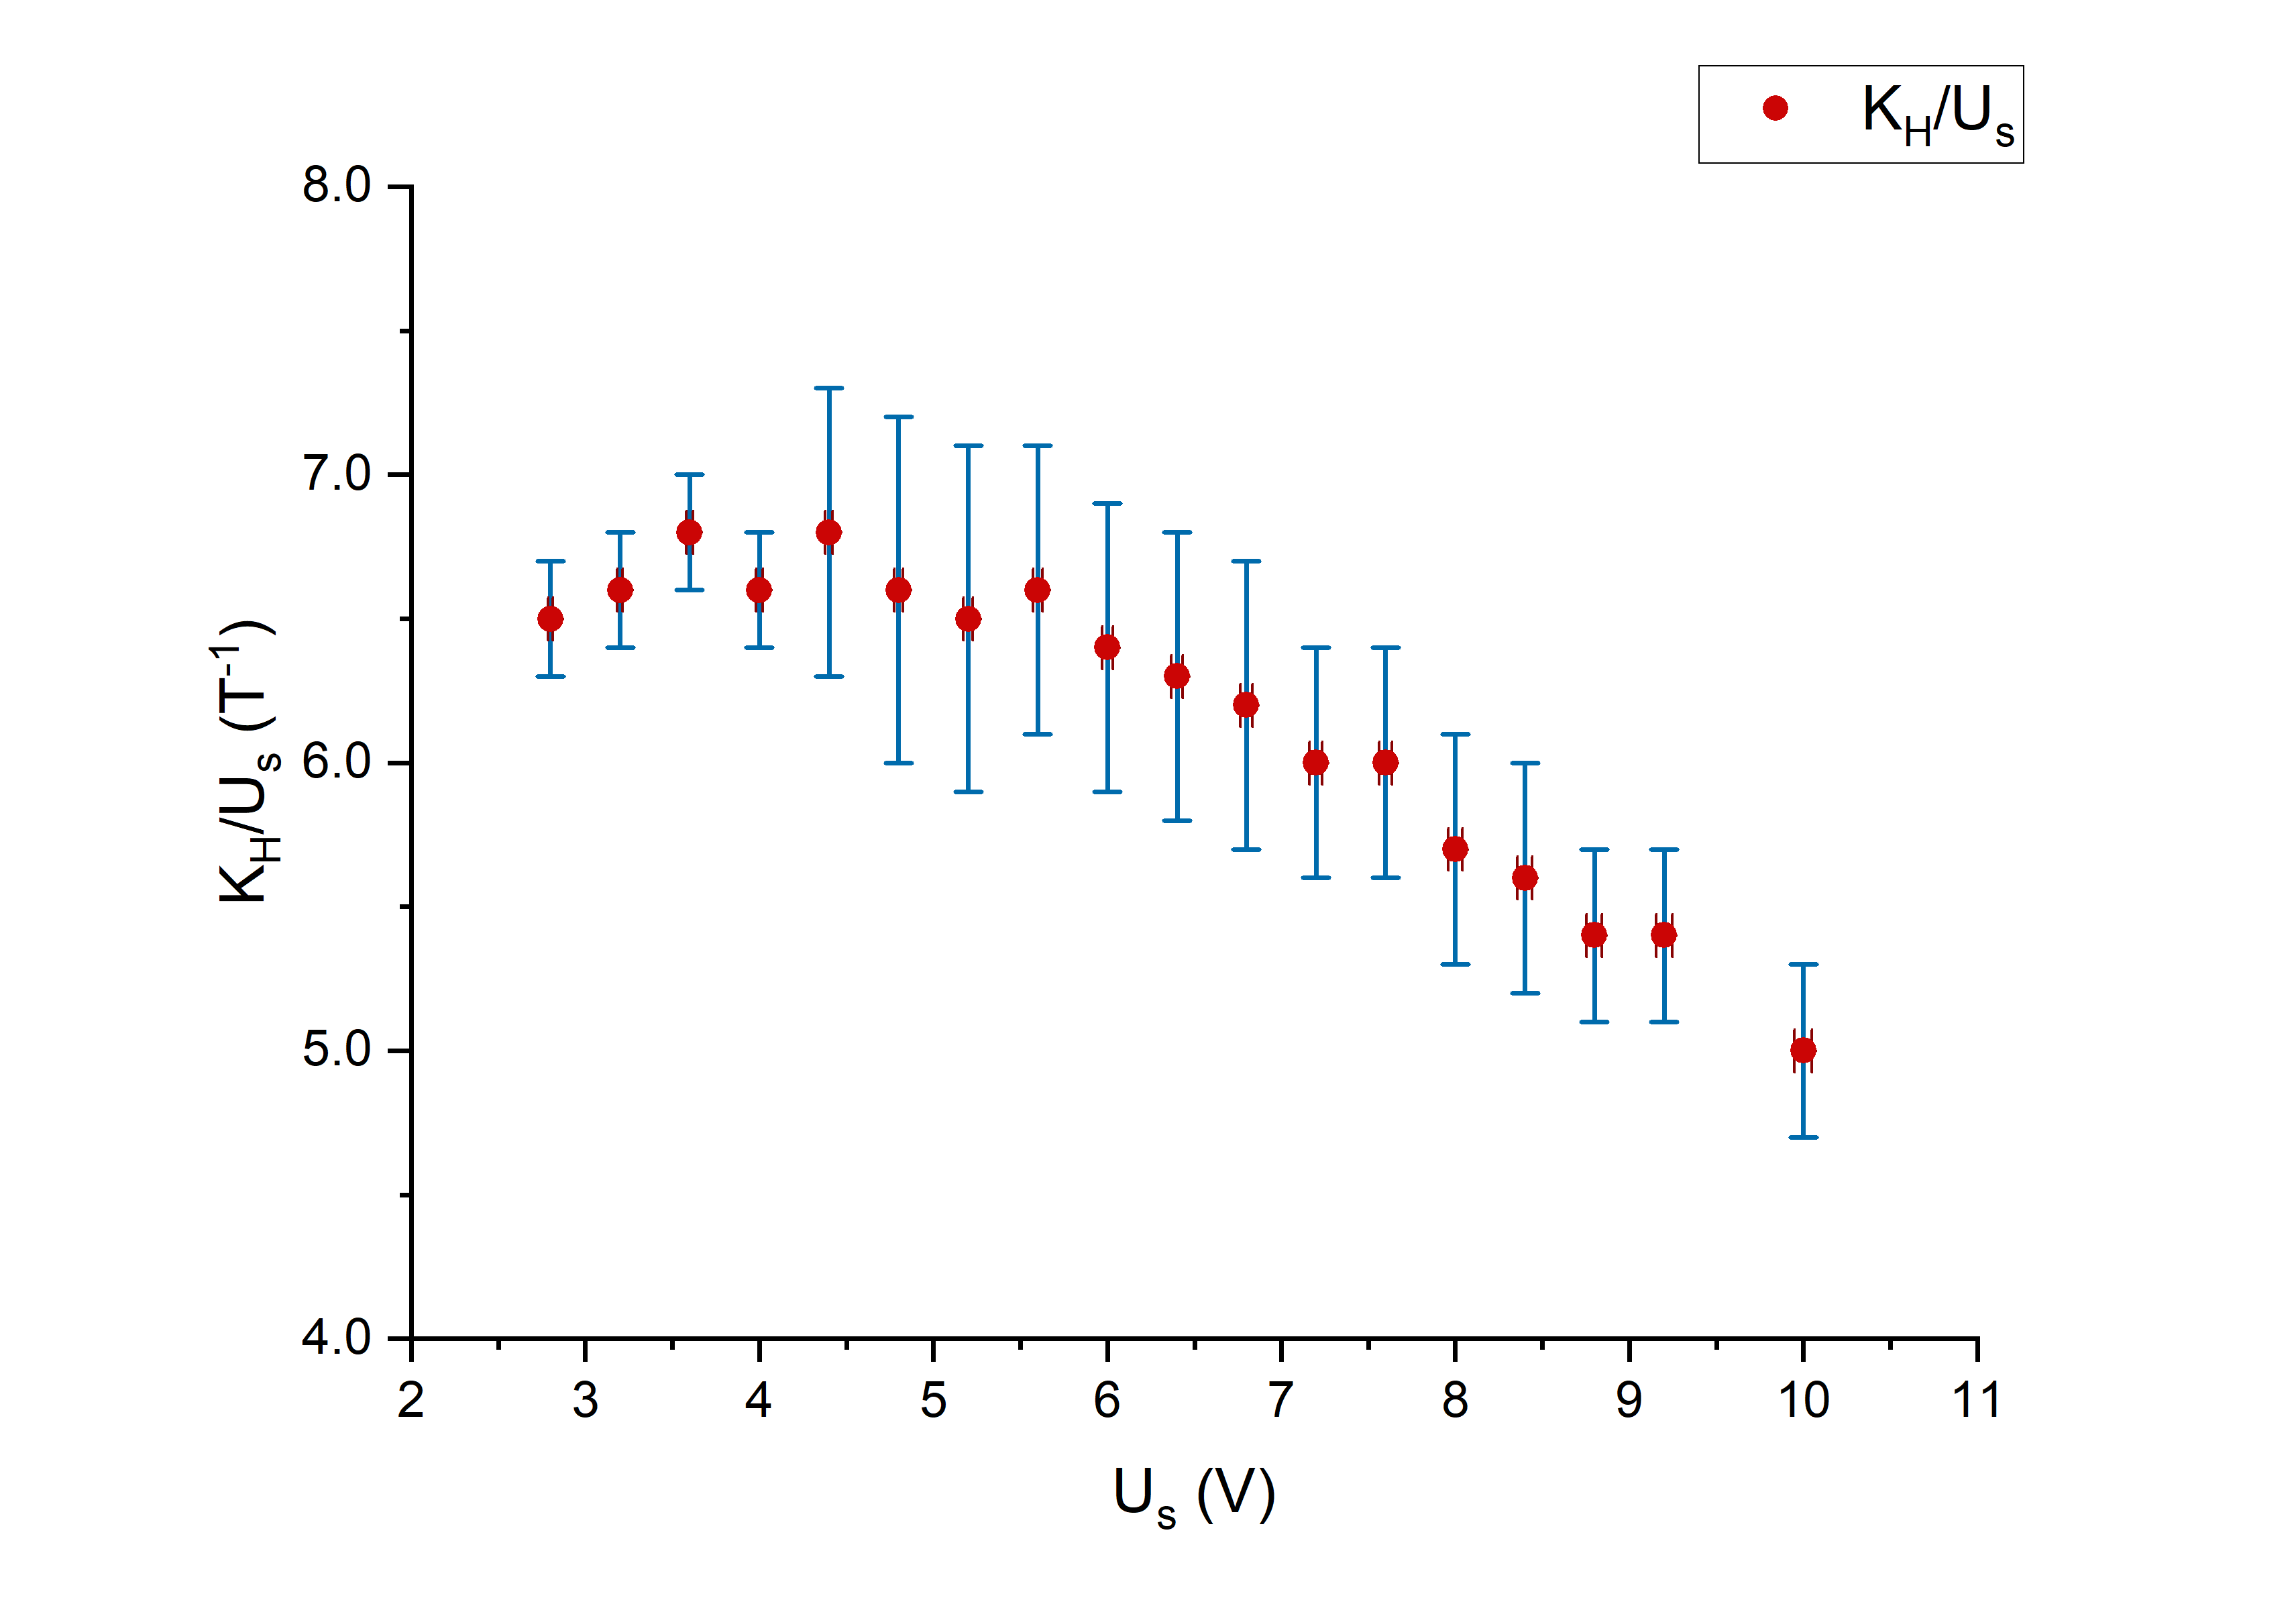
\includegraphics[width=0.75\textwidth]{KHUS.png}
	\caption{The $K_H/U_S$ vs. $U_S$ relation}
	\label{fig::KHUS}
\end{figure}

\subsection{Relation Between Output Voltage $U$ and Magnetic Field $B$}\label{sec::e2}

\textit{In this experiment, we will not take the magnetic field B into consideration when it comes to uncertainty, as requested.}

According to Eq.(\ref{eq::Bx}), $B$ is proportional to current $I_\text{M}$. We can obtain from Table \ref{table::theoretical value} that when $I_\text{M} = 100 \,\,\text{mA},$ $B(x=0,I_\text{M}=100\,[\text{mA}])=1.4366\times10^{-3}\,\,\text{T}.$ Therefore,
the theoretical value of the magnetic field is $$B(x=0) = \frac{I_\text{M}}{100}\times 1.4366\times10^{-3}.$$
Take the last set of data as an example,
$$B(x=0,I_\text{M}=0.50\,[\text{A}]) = \frac{1.4366\times10^{-3}}{100\times 10^{-3}}\times I_\text{M} = 7.2\times 10^{-3}\,[\text{T}].$$

It is noticed that the measured $U_{\text{out}}$ is the amplified output of $U_{H}$ and we supposed that $U = k \cdot U_{H}$. Then, theoretically, according to Eq. (\ref{eq::magnetic field}), we can derive that
$$B(x=0) = \frac{U-U_0}{K_\text{H}} = \frac{U_{\text{out}}}{K_\text{H}} = k\cdot\frac{U_\text{H}}{K_\text{H}},$$
where $k$ is a constant. Therefore, $B(x=0)$ is supposed to be proportional to the Hall voltage $U_\text{H}$.\\

The experimental results are shown in Table \ref{table::IMU}. By applying linear fit to the $I_\text{M}$ vs. $U$ plot (Fig.(\ref{fig::linear fit})), the slope of the curve
is then the measured sensitivity $K_{H}$, which is $33.6$ V/T, with uncertainty $0.7$ V/T. The measurement result of the sensitivity is then
$K_H = 33.6 \pm 0.7\,$V/T.

\begin{table}[H]
	\centering
	\begin{tabular}{clll}
		\hline
		   & $I_\text{M}\,\,[\text{A}] \pm 2\%\ [\text{A}]$ & \begin{tabular}[c]{@{}l@{}}$U_{\text{out}}\ [\text{mV}]\pm (0.05\%+$\\ $6\times10^{-3})\ [\text{mV}]$ \end{tabular} & $B(x=0)\ [\text{T}]$ \\
		\hline
		1  & 0 $\pm$ 0                                      & 0.83 $\pm$ 0.007           & 0                    \\
		2  & 0.05 $\pm$ 0.001                               & 30.08 $\pm$ 0.03           & 7.2$\times 10^{-4}$  \\
		3  & 0.10 $\pm$ 0.002                               & 51.32 $\pm$ 0.04           & 1.4$\times 10^{-3}$  \\
		4  & 0.15 $\pm$ 0.003                               & 73.38 $\pm$ 0.05           & 2.2$\times 10^{-3}$  \\
		5  & 0.20 $\pm$ 0.004                               & 97.71 $\pm$ 0.06           & 2.9$\times 10^{-3}$  \\
		6  & 0.25 $\pm$ 0.005                               & 121.64 $\pm$ 0.07          & 3.6$\times 10^{-3}$  \\
		7  & 0.30 $\pm$ 0.006                               & 143.67 $\pm$ 0.08          & 4.3$\times 10^{-3}$  \\
		8  & 0.35 $\pm$ 0.007                               & 166.63 $\pm$ 0.09          & 5.0$\times 10^{-3}$  \\
		9  & 0.40 $\pm$ 0.008                               & 187.79 $\pm$ 0.10          & 5.7$\times 10^{-3}$  \\
		10 & 0.45 $\pm$ 0.009                               & 210.10 $\pm$ 0.12          & 6.5$\times 10^{-3}$  \\
		11 & 0.50 $\pm$ 0.010                               & 231.1 $\pm$ 0.13           & 7.2$\times 10^{-3}$  \\
		\hline
	\end{tabular}
	\caption{Measurement data for the $I_\text{M}$ vs. $U$ relation and the calculated data for $B(x=0)$.}
	\label{table::IMU}
\end{table}

\begin{figure}[!htbp]
	\centering
	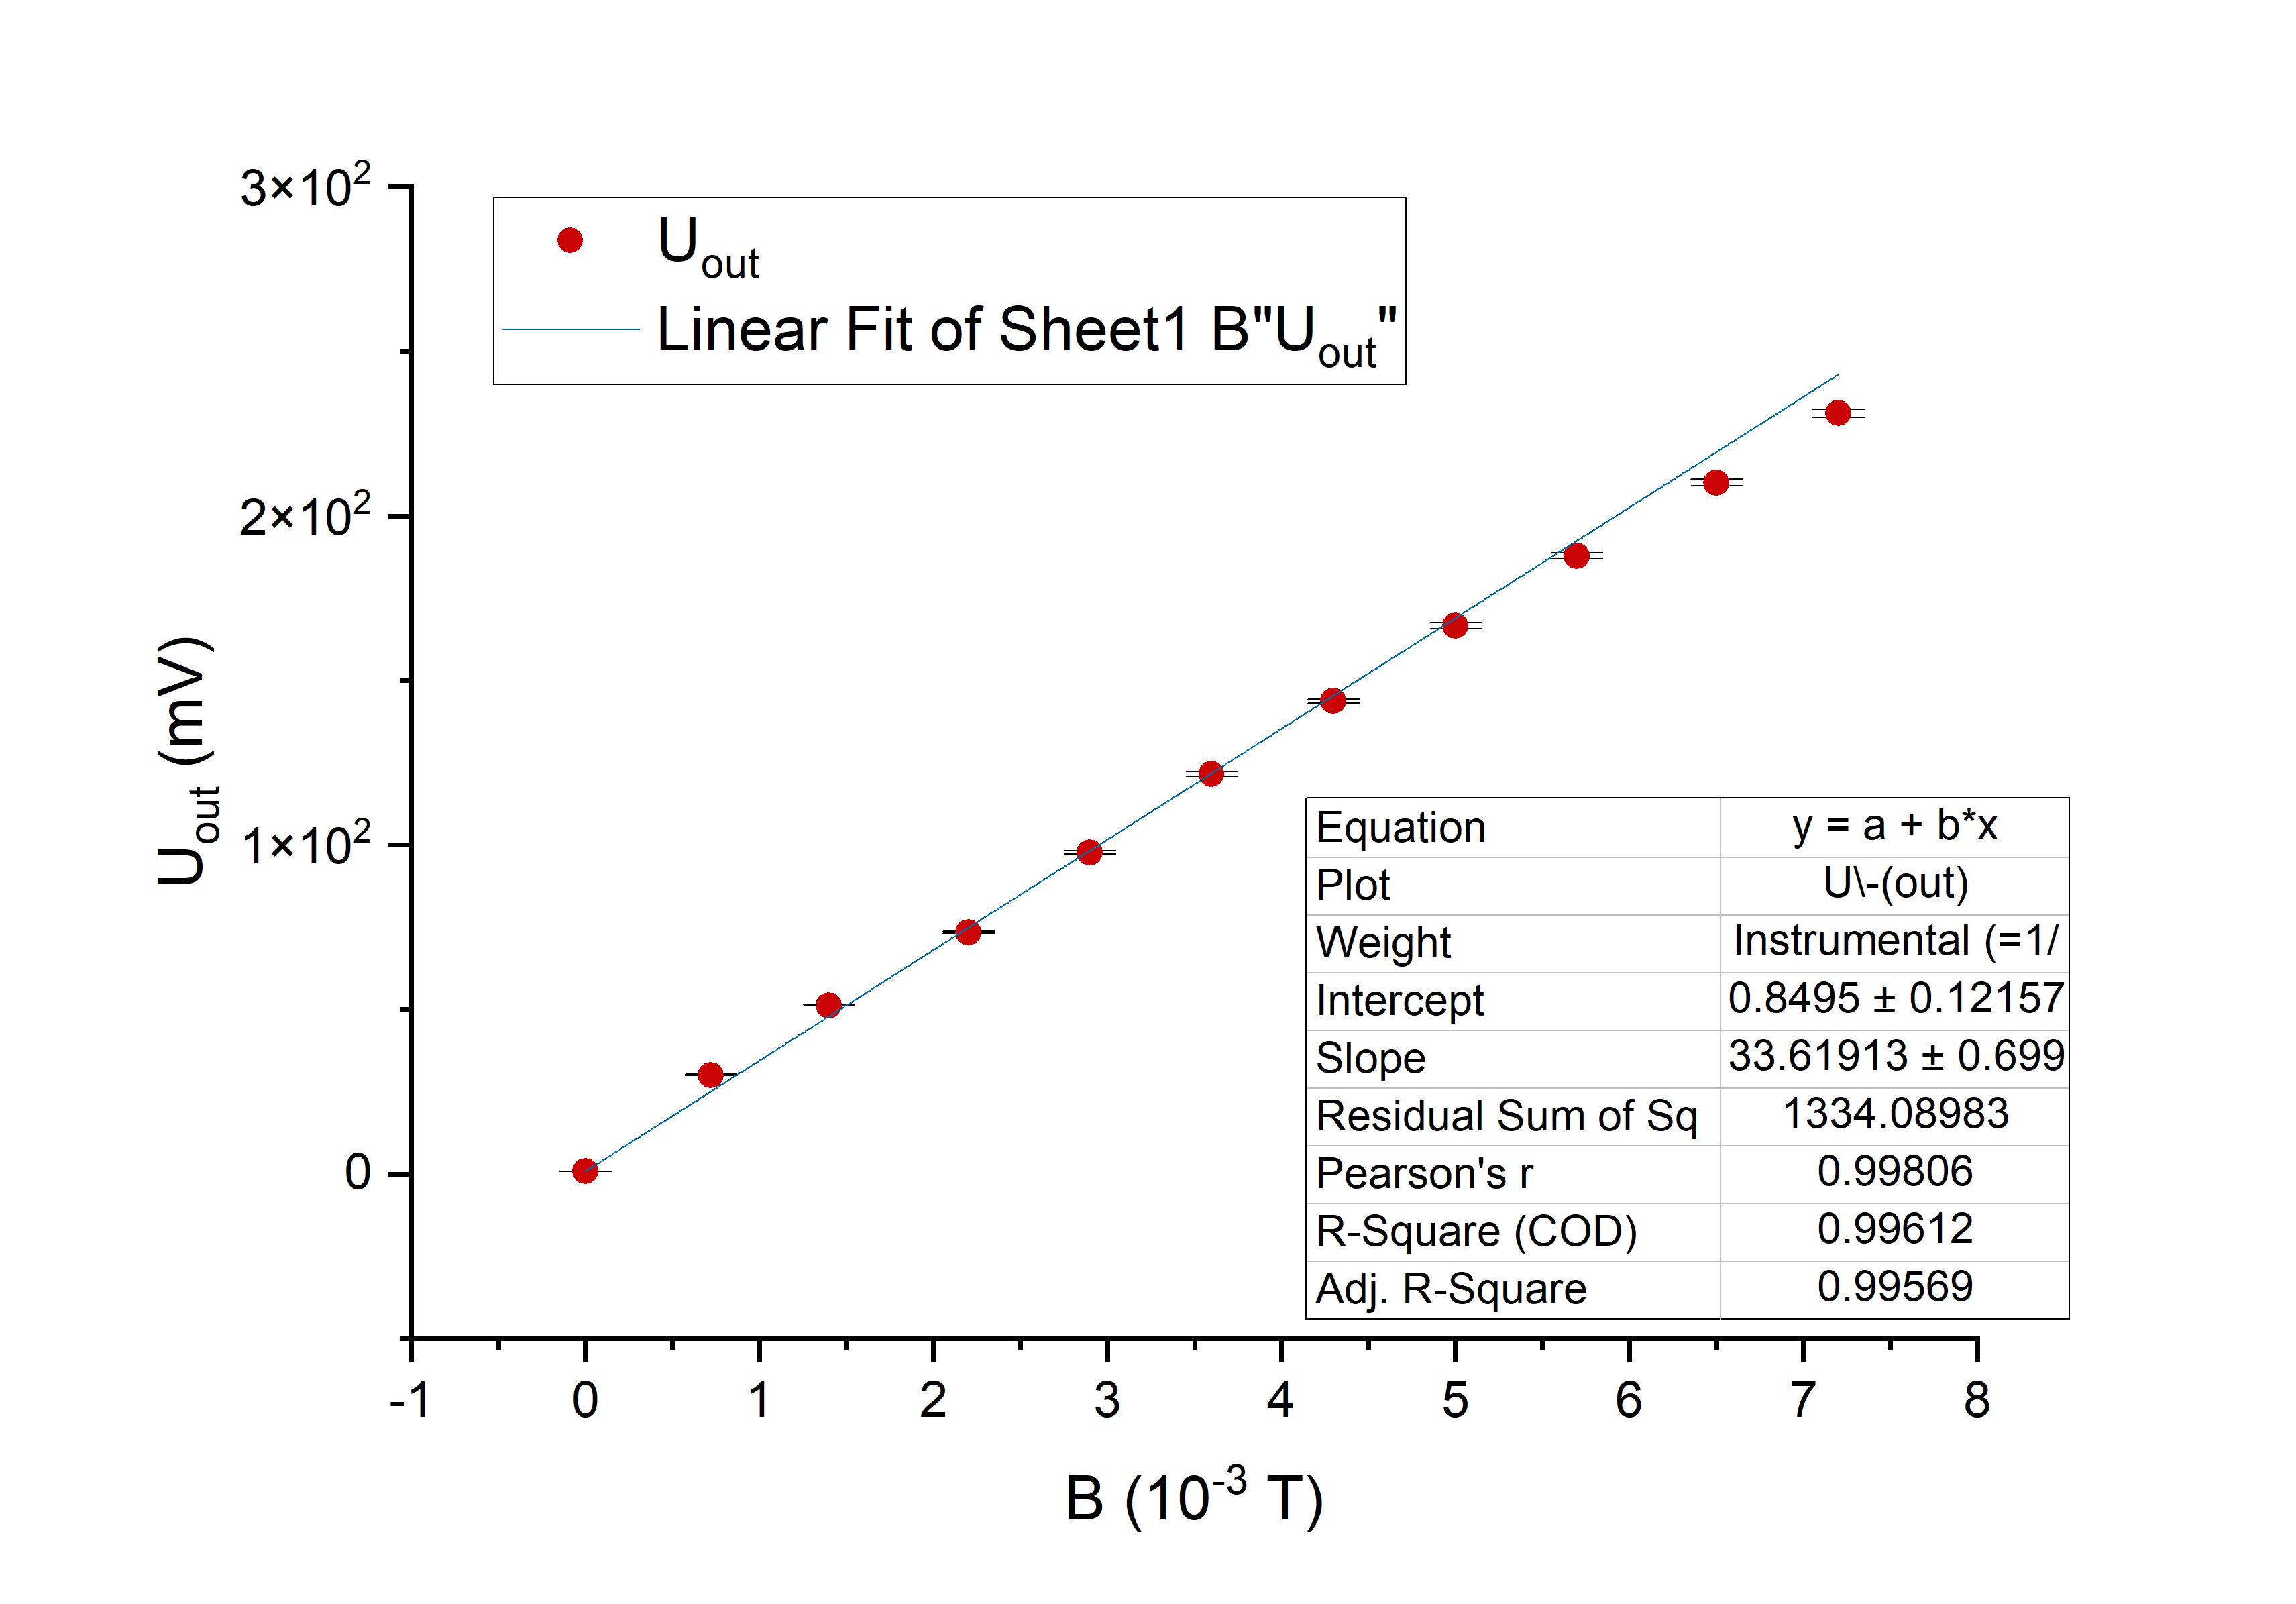
\includegraphics[width=0.8\textwidth]{linear fit.png}
	\caption{The linear fit of $U$ vs. $B$ relation}
	\label{fig::linear fit}
\end{figure}

\subsection{Magnetic Field Distribution Inside the Solenoid}

The measurement result of output voltage $U$ and the corresponding position $x$ are shown in Table \ref{TableUx}. According to Eq.(\ref{eq::magnetic field}) and the
measured value of $K_{H}$ in section \ref{sec::e2}, $B(x)$ can be obtained from $B(x) = \frac{U}{K_\text{H}} = \frac{U}{33.6}$
Take the first set of data as an example, $$B(x) = \frac{U}{K_\text{H}} = \frac{12.20\times 10^{-3}}{33.6} = (0.363 \pm 0.008) \times 10^{-3} \,\,[\text{T}].$$
The $B(x)$ are calculated for each set of data and the results are shown in Table \ref{TableBx}.

\begin{table}[htbp]
	\centering
	\begin{tabular}{ccc||ccc}
		\hline
		   & $x$[cm]$\pm$0.05[cm] & $U$[mV]$\pm$(0.05$\%$+$6 \times 10^{-3})[\text{mV}]$ &    & $x$[cm]$\pm$0.05[cm] & $U$[mV]$\pm$(0.05$\%$+$6 \times 10^{-3})[\text{mV}]$ \\
		\hline
		1  & 0.00                 & 12.20 $\pm$ 0.012                                    & 27 & 16.00                & 118.14 $\pm$ 0.07                                    \\
		2  & 0.50                 & 15.27 $\pm$ 0.014                                    & 28 & 17.00                & 118.12 $\pm$ 0.07                                    \\
		3  & 1.00                 & 20.64 $\pm$ 0.016                                    & 29 & 18.00                & 118.04 $\pm$ 0.07                                    \\
		4  & 1.50                 & 27.95 $\pm$ 0.02                                     & 30 & 19.00                & 117.93 $\pm$ 0.07                                    \\
		5  & 2.00                 & 39.47 $\pm$ 0.03                                     & 31 & 20.00                & 117.87 $\pm$ 0.07                                    \\
		6  & 2.50                 & 54.53 $\pm$ 0.04                                     & 32 & 21.00                & 117.48 $\pm$ 0.07                                    \\
		7  & 3.00                 & 71.20 $\pm$ 0.05                                     & 33 & 22.00                & 117.27 $\pm$ 0.07                                    \\
		8  & 3.50                 & 86.03 $\pm$ 0.05                                     & 34 & 23.00                & 116.52 $\pm$ 0.07                                    \\
		9  & 4.00                 & 96.45 $\pm$ 0.06                                     & 35 & 24.00                & 115.35 $\pm$ 0.07                                    \\
		10 & 4.50                 & 103.35 $\pm$ 0.06                                    & 36 & 25.00                & 113.25 $\pm$ 0.07                                    \\
		11 & 5.00                 & 107.76 $\pm$ 0.06                                    & 37 & 26.00                & 109.47 $\pm$ 0.06                                    \\
		12 & 5.50                 & 110.62 $\pm$ 0.07                                    & 38 & 27.00                & 101.05 $\pm$ 0.06                                    \\
		13 & 6.00                 & 112.67 $\pm$ 0.07                                    & 39 & 27.20                & 98.40 $\pm$ 0.06                                     \\
		14 & 6.50                 & 113.90 $\pm$ 0.07                                    & 40 & 27.60                & 91.27 $\pm$ 0.06                                     \\
		15 & 7.00                 & 114.90 $\pm$ 0.07                                    & 41 & 27.80                & 87.47 $\pm$ 0.05                                     \\
		16 & 7.50                 & 115.56 $\pm$ 0.07                                    & 42 & 28.00                & 82.41 $\pm$ 0.05                                     \\
		17 & 8.00                 & 116.18 $\pm$ 0.07                                    & 43 & 28.20                & 75.95 $\pm$ 0.05                                     \\
		18 & 8.50                 & 116.71 $\pm$ 0.07                                    & 44 & 28.40                & 69.49 $\pm$ 0.05                                     \\
		19 & 9.00                 & 117.20 $\pm$ 0.07                                    & 45 & 28.60                & 62.78 $\pm$ 0.04                                     \\
		20 & 9.50                 & 117.28 $\pm$ 0.07                                    & 46 & 28.80                & 56.25 $\pm$ 0.04                                     \\
		21 & 10.00                & 117.67 $\pm$ 0.07                                    & 47 & 29.00                & 49.60 $\pm$ 0.04                                     \\
		22 & 11.00                & 117.87 $\pm$ 0.07                                    & 48 & 29.20                & 43.65 $\pm$ 0.03                                     \\
		23 & 12.00                & 118.02 $\pm$ 0.07                                    & 49 & 29.40                & 37.75 $\pm$ 0.03                                     \\
		24 & 13.00                & 118.12 $\pm$ 0.07                                    & 50 & 29.60                & 32.68 $\pm$ 0.03                                     \\
		25 & 14.00                & 118.01 $\pm$ 0.07                                    & 51 & 29.80                & 28.52 $\pm$ 0.03                                     \\
		26 & 15.00                & 118.19 $\pm$ 0.07                                    & 52 & 30.00                & 25.57 $\pm$ 0.019                                    \\
		\hline
	\end{tabular}
	\caption{Data for the $U$ vs. $x$ relation}\label{TableUx}
\end{table}

\begin{table}[H]
	\centering
	\begin{tabular}{ccc||ccc}
		\hline
		   & $x\,\,[\text{cm}] \pm 0.05\,\,[\text{cm}]$ & $B(x)\,\,[10^{-3}\,\,\text{T}]$ &    & $x\,\,[\text{cm}] \pm 0.05\,\,[\text{cm}]$ & $B(x)\,\,[10^{-3}\,\,\text{T}]$ \\
		\hline
		1  & 0.00                                       & 0.363 $\pm$ 0.008               & 27 & 16.00                                      & 3.47 $\pm$ 0.08                 \\
		2  & 0.50                                       & 0.449 $\pm$ 0.010               & 28 & 17.00                                      & 3.47 $\pm$ 0.08                 \\
		3  & 1.00                                       & 0.607 $\pm$ 0.013               & 29 & 18.00                                      & 3.47 $\pm$ 0.08                 \\
		4  & 1.50                                       & 0.822 $\pm$ 0.017               & 30 & 19.00                                      & 3.47 $\pm$ 0.08                 \\
		5  & 2.00                                       & 1.16 $\pm$ 0.03                 & 31 & 20.00                                      & 3.47 $\pm$ 0.08                 \\
		6  & 2.50                                       & 1.60 $\pm$ 0.04                 & 32 & 21.00                                      & 3.46 $\pm$ 0.08                 \\
		7  & 3.00                                       & 2.09 $\pm$ 0.05                 & 33 & 22.00                                      & 3.45 $\pm$ 0.08                 \\
		8  & 3.50                                       & 2.53 $\pm$ 0.06                 & 34 & 23.00                                      & 3.43 $\pm$ 0.07                 \\
		9  & 4.00                                       & 2.83 $\pm$ 0.06                 & 35 & 24.00                                      & 3.39 $\pm$ 0.07                 \\
		10 & 4.50                                       & 3.04 $\pm$ 0.07                 & 36 & 25.00                                      & 3.33 $\pm$ 0.07                 \\
		11 & 5.00                                       & 3.17 $\pm$ 0.07                 & 37 & 26.00                                      & 3.22 $\pm$ 0.07                 \\
		12 & 5.50                                       & 3.25 $\pm$ 0.07                 & 38 & 27.00                                      & 2.97 $\pm$ 0.07                 \\
		13 & 6.00                                       & 3.31 $\pm$ 0.07                 & 39 & 27.20                                      & 2.89 $\pm$ 0.06                 \\
		14 & 6.50                                       & 3.35 $\pm$ 0.07                 & 40 & 27.60                                      & 2.68 $\pm$ 0.06                 \\
		15 & 7.00                                       & 3.38 $\pm$ 0.07                 & 41 & 27.80                                      & 2.57 $\pm$ 0.06                 \\
		16 & 7.50                                       & 3.40 $\pm$ 0.07                 & 42 & 28.00                                      & 2.42 $\pm$ 0.05                 \\
		17 & 8.00                                       & 3.42 $\pm$ 0.07                 & 43 & 28.20                                      & 2.23 $\pm$ 0.05                 \\
		18 & 8.50                                       & 3.43 $\pm$ 0.07                 & 44 & 28.40                                      & 2.04 $\pm$ 0.05                 \\
		19 & 9.00                                       & 3.45 $\pm$ 0.07                 & 45 & 28.60                                      & 1.85 $\pm$ 0.04                 \\
		20 & 9.50                                       & 3.45 $\pm$ 0.08                 & 46 & 28.80                                      & 1.65 $\pm$ 0.04                 \\
		21 & 10.00                                      & 3.46 $\pm$ 0.08                 & 47 & 29.00                                      & 1.46 $\pm$ 0.03                 \\
		22 & 11.00                                      & 3.47 $\pm$ 0.08                 & 48 & 29.20                                      & 1.28 $\pm$ 0.03                 \\
		23 & 12.00                                      & 3.47 $\pm$ 0.08                 & 49 & 29.40                                      & 1.11 $\pm$ 0.03                 \\
		24 & 13.00                                      & 3.47 $\pm$ 0.08                 & 50 & 29.60                                      & 0.96 $\pm$ 0.02                 \\
		25 & 14.00                                      & 3.47 $\pm$ 0.08                 & 51 & 29.80                                      & 0.839 $\pm$ 0.018               \\
		26 & 15.00                                      & 3.48 $\pm$ 0.08                 & 52 & 30.00                                      & 0.752 $\pm$0.016                \\
		\hline
	\end{tabular}
	\caption{Data for the $B(x)$ vs. $x$ relation.}\label{TableBx}
\end{table}

The theoretical curve of the magnetic field distribution inside the solenoid can be obtained from Eq.\eqref{eq::Bx} and the data in Table \ref{table::theoretical value}, by multiplying the data in the table by $\frac{250}{100} = 2.5$, since we have set the current as 250 mA instead of 100 mA.

Then we plot the theoretical curve together with the measured value of the magnetic field distribution in Fig.(\ref{fig::theo_and_meas}). 
The origin of the plot is set at the center of the solenoid, thus $15$ cm are subtracted from the $x$ in the measurement data.

\begin{figure}[!htbp]
	\centering
	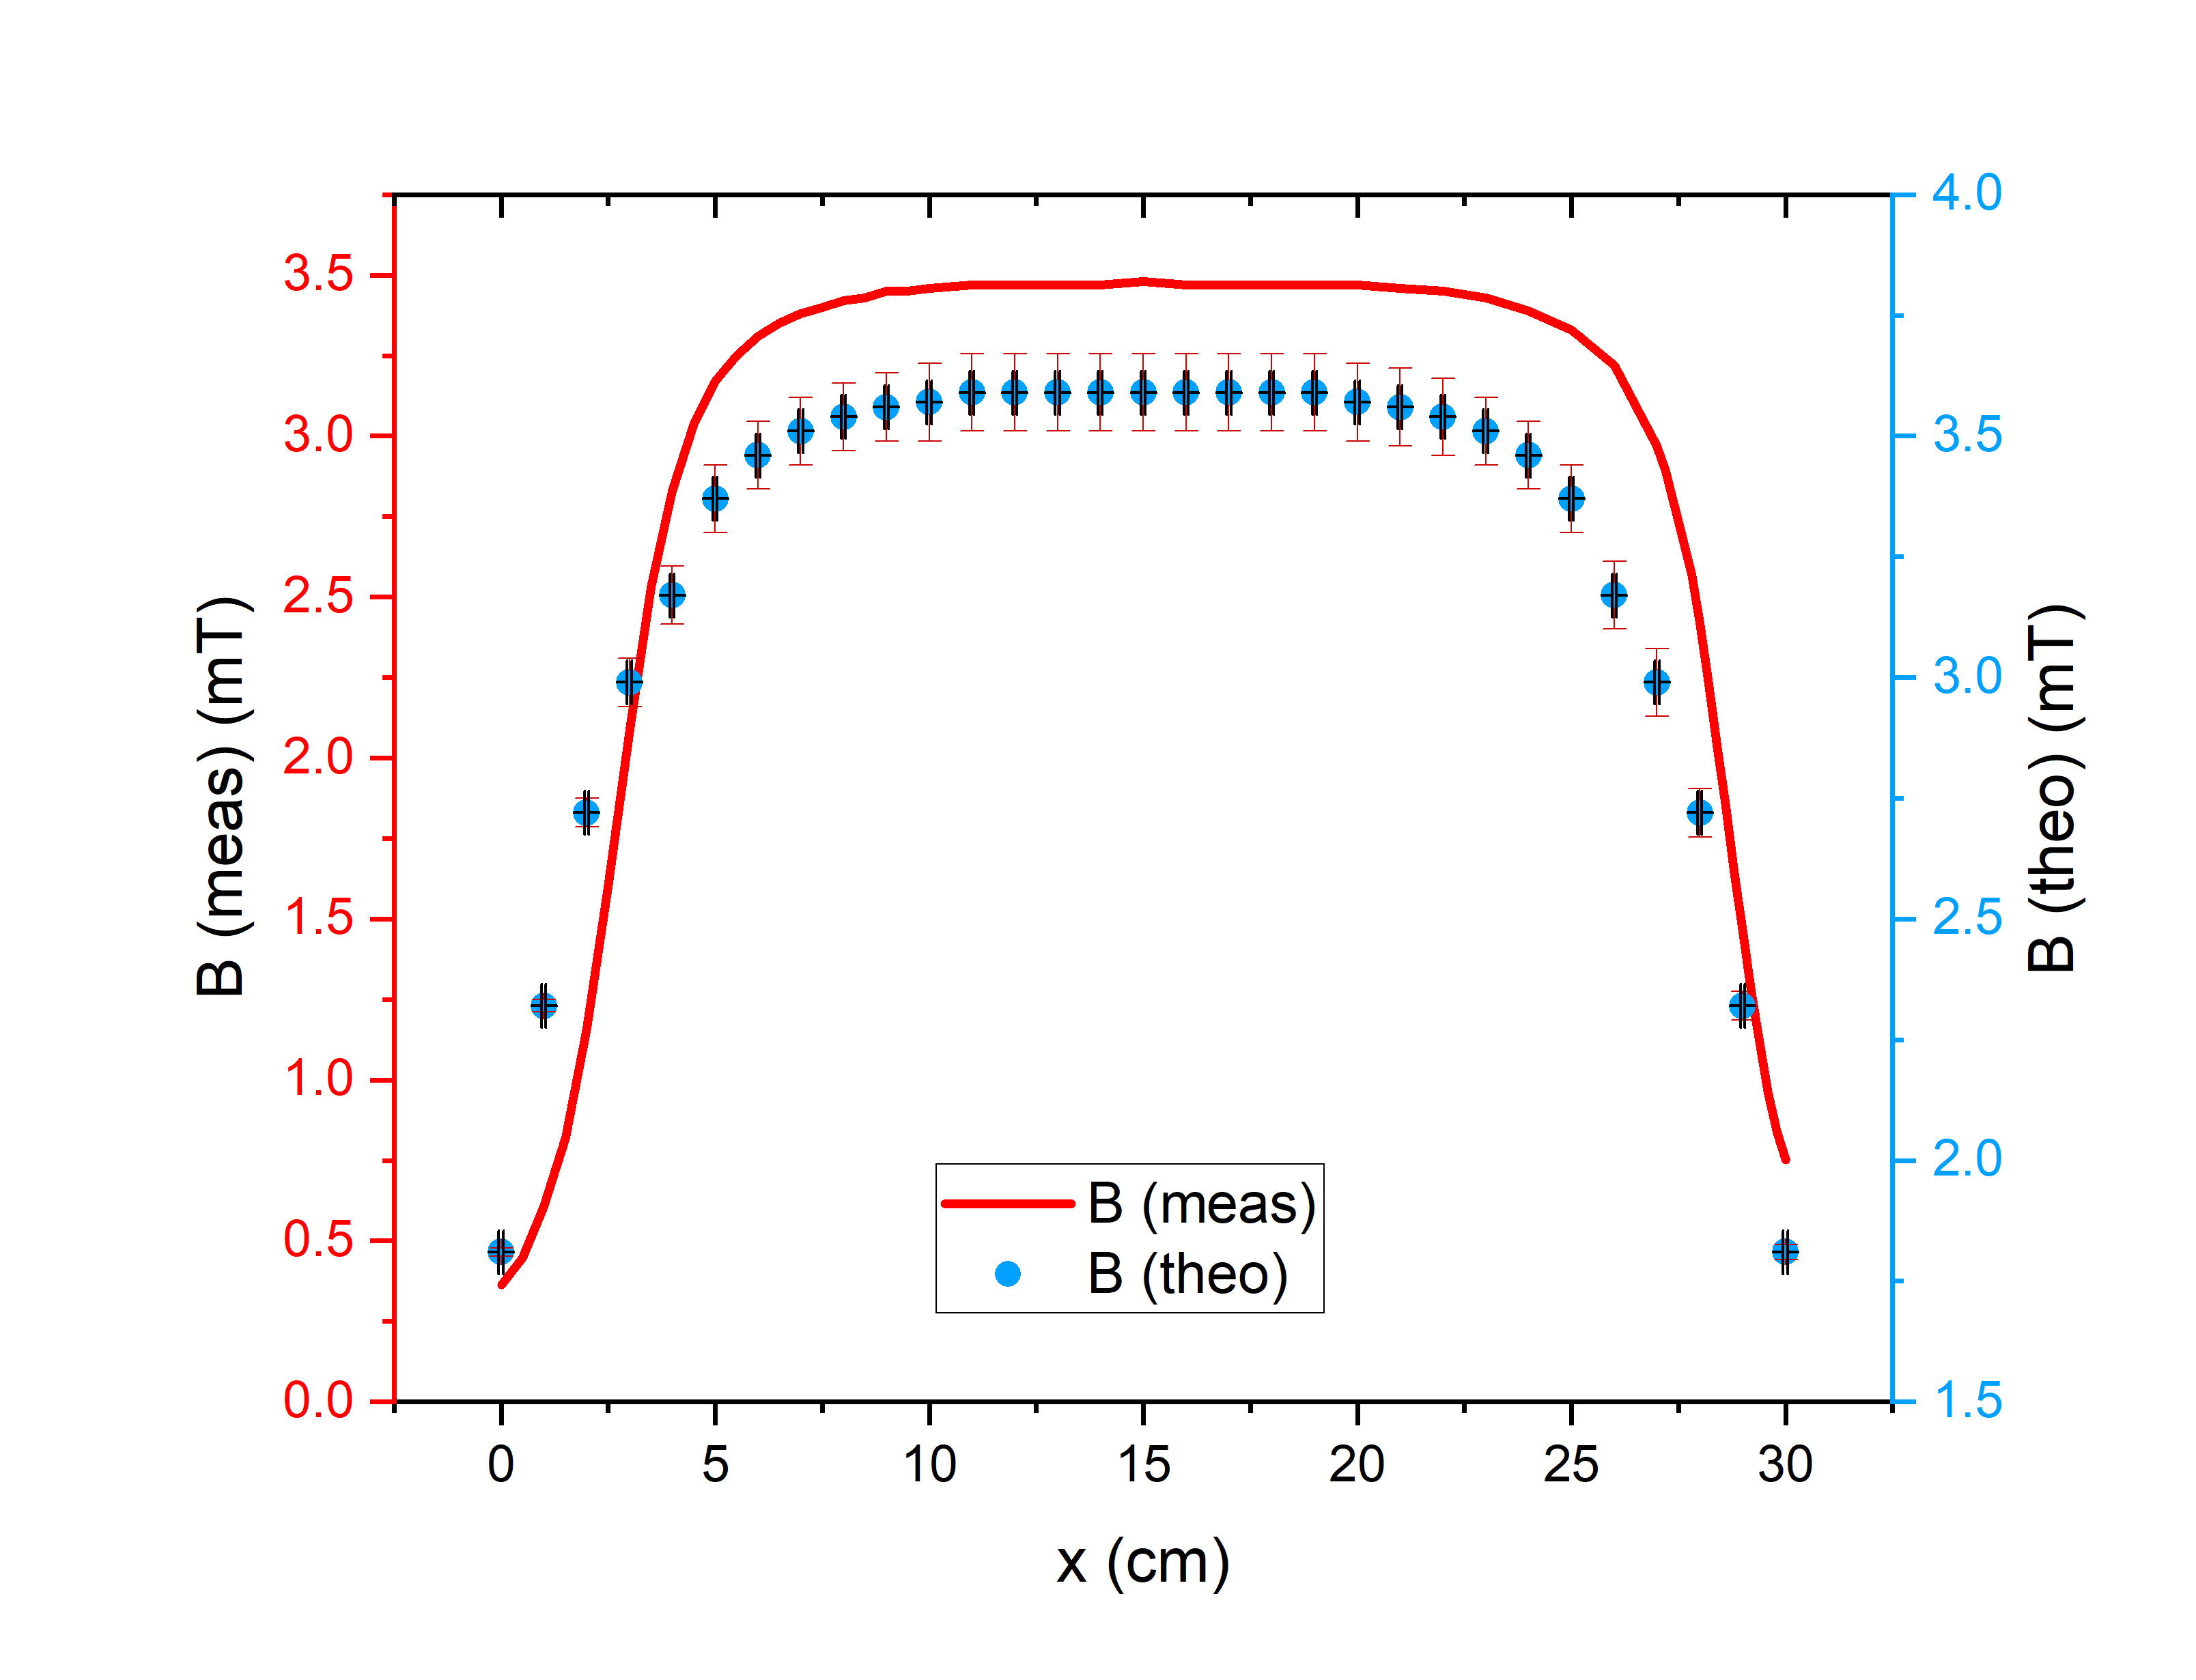
\includegraphics[width=0.8\textwidth]{theo_and_meas.png}
	\caption{Measured and theoretical magnetic field distribution inside the solenoid.}
	\label{fig::theo_and_meas}
\end{figure}


\section{Uncertainty Analysis}

\subsection{Relationship Between Sensitivity $K_H$ and Working Voltage $U_S$}
According to Table \ref{table::initial}, the uncertainties are calculated as
\begin{align*}
	u_{U_\text{S}}  & = 5.00\times 0.5\% = 0.03\ [\text{V}]                          \\
	u_{U_0}         & = 2.504\times0.05\%+6\times10^{-3} = 0.007\ [\text{V}]         \\
	u_U             & = 2.621\times0.05\%+6\times10^{-3} = 0.007\ [\text{V}]         \\
	u_{I_\text{M2}} & = 250 \times 10^{-3} \times 2\% = 5 \times 10^{-3}\ [\text{A}]
\end{align*}
while $B(x=0,I_\text{M}=250\ [\text{mA}]) = \frac{I_\text{M2}}{I_{\text{M1}}} \times B(x=0,I_\text{M}=100\ [\text{mA}])$
\begin{equation*}
	u_B = \frac{B(x=0,I_\text{M}=100\ [\text{mA}])}{I_{\text{M1}}}u_{I_\text{M2}} = \frac{1.4366\times 10^{-3}}{100\times 10^{-3}} \times 5\times 10^{-3} = 7 \times 10^{-5}\ [\text{T}]
\end{equation*}
\par Then for $K_\text{H} = \frac{U-U_0}{B}$, its uncertainty is
\begin{align*}
	u_{K_\text{H}} & = \sqrt{(\frac{\partial K_\text{H}}{\partial U}u_U)^2+(\frac{\partial K_\text{H}}{\partial U_0}u_{U_0})^2+(\frac{\partial K_\text{H}}{\partial B}u_B)^2} = \sqrt{(\frac{u_U}{B})^2+(\frac{-u_{U_0}}{B})^2+(-\frac{(U-U_0)u_B}{B^2})^2} \\
	               & =\sqrt{(\frac{0.007}{1.4366\times10^{-3}\times250/100})^2+(\frac{-0.007}{1.4366\times10^{-3}\times250/100})^2+(\frac{(2.621-2.504)\times 7\times 10^{-5}}{(1.4366\times10^{-3}\times250/100)^2})^2}                                    \\
	               & =3\ [\text{V}/\text{T}].
\end{align*}

For Table \ref{table::e1}, the uncertainties of data for voltage measurements are calculated as follows. Take the first set of data as an example,
$$u_{U_\text{S}} = 2.80\times 0.5\% = 0.014\,\,[\text{V}],$$
$$u_{U_0} = 1.4004\times0.05\%+6\times10^{-4} = 0.0013\,\,[\text{V}],$$
$$u_U = 1.4656\times0.05\%+6\times10^{-4} = 0.0014\,\,[\text{V}].$$

The uncertainty for $ K_\text{H}/U_\text{S} = \frac{U-U_0}{BU_\text{S}} $ is calculated as
\begin{align*}
	u_{K_\text{H}/U_\text{S}} & = \sqrt{(\frac{\partial K_\text{H}/U_\text{S}}{\partial U}u_U)^2+(\frac{\partial K_\text{H}/U_\text{S}}{\partial U_0}u_{U_0})^2+(\frac{\partial K_\text{H}/U_\text{S}}{\partial U_\text{S}}u_{U_\text{S}})^2+(\frac{\partial K_\text{H}/U_\text{S}}{\partial B}u_B)^2} \\
	                          & = \sqrt{(\frac{u_U}{BU_\text{S}})^2+(\frac{-u_{U_0}}{BU_\text{S}})^2+(-\frac{U-U_0}{BU_\text{S}^2}u_{U_\text{S}})^2+(-\frac{U-U_0}{B^2U_\text{S}}u_{B})^2}                                                                                                             \\
	                          & = \sqrt{(\frac{0.0014}{3.59\times10^{-3}\times2.80})^2+(\frac{-0.0013}{3.59\times10^{-3} \times2.80})^2+(-\frac{(1.4656-1.4004)\times 0.014}{3.59\times10^{-3} \times 2.80^2})^2+(-\frac{(1.4656-1.4004)\times 7\times 10^{-5}}{{(3.59\times 10^{-3})}^2 \times 2.80}} \\
	                          & =0.2\ [\text{T}^{-1}].
\end{align*}

The uncertainties of all other data in Table \ref{table::e1} are calculated in this way and the results are presented in Table \ref{table::ue1}.

\begin{table}[H]
	\centering
	\begin{tabular}{crrrc}
		\hline
		   & $u_{U_\text{S}}\,\,[\text{V}]$ & $u_{U_0}\,\,[\text{V}]$ & $u_U\,\,[\text{V}]$ & $u_{K_\text{H}/U_\text{S}}\,\,[\text{T}^{-1}]$ \\
		\hline
		1  & 0.014                          & 0.0013                  & 0.0014              & 0.2                                            \\
		2  & 0.016                          & 0.0014                  & 0.0015              & 0.2                                            \\
		3  & 0.018                          & 0.0015                  & 0.0016              & 0.2                                            \\
		4  & 0.020                          & 0.007                   & 0.007               & 0.2                                            \\
		5  & 0.022                          & 0.008                   & 0.008               & 0.5                                            \\
		6  & 0.024                          & 0.008                   & 0.008               & 0.6                                            \\
		7  & 0.026                          & 0.008                   & 0.008               & 0.6                                            \\
		8  & 0.028                          & 0.008                   & 0.008               & 0.5                                            \\
		9  & 0.030                          & 0.008                   & 0.008               & 0.5                                            \\
		10 & 0.032                          & 0.008                   & 0.008               & 0.5                                            \\
		11 & 0.034                          & 0.008                   & 0.008               & 0.5                                            \\
		12 & 0.036                          & 0.008                   & 0.008               & 0.4                                            \\
		13 & 0.038                          & 0.008                   & 0.008               & 0.4                                            \\
		14 & 0.040                          & 0.008                   & 0.008               & 0.4                                            \\
		15 & 0.042                          & 0.008                   & 0.009               & 0.4                                            \\
		16 & 0.044                          & 0.009                   & 0.009               & 0.3                                            \\
		17 & 0.046                          & 0.009                   & 0.009               & 0.3                                            \\
		18 & 0.050                          & 0.009                   & 0.009               & 0.3                                            \\
		\hline
	\end{tabular}
	\caption{Uncertainties of data in Table \ref{table::e1}.}
	\label{table::ue1}
\end{table}

\subsection{Uncertainty of Input Current $I_\text{M}$, Output Voltage $U$ and Magnetic Field $B$}

Take the last set of data in Table \ref{table::IMU} as an example.\\

The uncertainty for $I_\text{M}$ is
$$u_{I_\text{M}} = 0.50\times 2\% = 0.010\,\,[\text{A}]$$

The uncertainty for $U$ is
$$u_U = 231.1\times 0.05\%+6\times10^{-3} = 0.12\,\,[\text{mV}].$$

The uncertainties of all other data in Table \ref{table::IMU} are calculated in this way are the results are presented in Table \ref{table::uIMU}.

\begin{table}[H]
	\centering
	\begin{tabular}{ccc}
		\hline
		   & $u_{I_\text{M}}\,\,[\text{A}]$ & $u_{U_{\text{out}}}\,\,[\text{V}]$ \\
		\hline
		1  & 0                              & 0.007                              \\
		2  & 0.001                          & 0.03                               \\
		3  & 0.002                          & 0.04                               \\
		4  & 0.003                          & 0.05                               \\
		5  & 0.004                          & 0.06                               \\
		6  & 0.005                          & 0.07                               \\
		7  & 0.006                          & 0.08                               \\
		8  & 0.007                          & 0.09                               \\
		9  & 0.008                          & 0.10                               \\
		10 & 0.009                          & 0.12                               \\
		11 & 0.010                          & 0.13                               \\
		\hline
	\end{tabular}
	\caption{Uncertainty of data in Table \ref{table::IMU}.}
	\label{table::uIMU}
\end{table}

\subsection{Uncertainty of Magnetic Field Inside the Solenoid Measurement}

The uncertainty of position measurement is 0.05 cm.

As for the uncertainty of the output voltage, taking the first set of data as an example,
$$u_U = 12.20 \times 0.05\% + 6\times 10^{-3} = 0.012\ \text{[mV]}$$

Due to $B(x) =\frac{U}{K_\text{H}}$,
$$ u_B = \sqrt{(\frac{\partial B}{\partial U}u_U)^2 + (\frac{\partial B}{\partial K_\text{H}}u_{K_\text{H}})^2} = \sqrt{(\frac{u_U}{K_\text{H}})^2 + (-\frac{U}{K_\text{H}^2}u_{K_\text{H}})^2}. $$

Taking the first set of data as an example,
$$  u_B = \sqrt{(\frac{0.012\times 10^{-3}}{33.6})^2 + (-\frac{12.20\times 10^{-3}}{33.6^2}\times 0.7)^2} = 0.008 \times10^{-3}\,[\text{T}]. $$

The uncertainties for all other sets of data are calculated and shown in Table \ref{table::uUB}.

\begin{table}[htbp]
	\centering
	\begin{tabular}{ccc||ccc}
		\hline
		   & $u_U\,\,[\text{mV}]$ & $B(x)\,\,[10^{-3}\,\,\text{T}]$ &    & $u_U\,\,[\text{mV}]$ & $B(x)\,\,[10^{-3}\,\,\text{T}]$ \\
		\hline
		1  & 0.012                & 0.008                           & 27 & 0.07                 & 0.08                            \\
		2  & 0.014                & 0.010                           & 28 & 0.07                 & 0.08                            \\
		3  & 0.016                & 0.013                           & 29 & 0.07                 & 0.08                            \\
		4  & 0.02                 & 0.017                           & 30 & 0.07                 & 0.08                            \\
		5  & 0.03                 & 0.03                            & 31 & 0.07                 & 0.08                            \\
		6  & 0.04                 & 0.04                            & 32 & 0.07                 & 0.08                            \\
		7  & 0.05                 & 0.05                            & 33 & 0.07                 & 0.08                            \\
		8  & 0.05                 & 0.06                            & 34 & 0.07                 & 0.07                            \\
		9  & 0.06                 & 0.06                            & 35 & 0.07                 & 0.07                            \\
		10 & 0.06                 & 0.07                            & 36 & 0.07                 & 0.07                            \\
		11 & 0.06                 & 0.07                            & 37 & 0.06                 & 0.07                            \\
		12 & 0.07                 & 0.07                            & 38 & 0.06                 & 0.07                            \\
		13 & 0.07                 & 0.07                            & 39 & 0.06                 & 0.06                            \\
		14 & 0.07                 & 0.07                            & 40 & 0.06                 & 0.06                            \\
		15 & 0.07                 & 0.07                            & 41 & 0.05                 & 0.06                            \\
		16 & 0.07                 & 0.07                            & 42 & 0.05                 & 0.05                            \\
		17 & 0.07                 & 0.07                            & 43 & 0.05                 & 0.05                            \\
		18 & 0.07                 & 0.07                            & 44 & 0.05                 & 0.05                            \\
		19 & 0.07                 & 0.07                            & 45 & 0.04                 & 0.04                            \\
		20 & 0.07                 & 0.08                            & 46 & 0.04                 & 0.04                            \\
		21 & 0.07                 & 0.08                            & 47 & 0.04                 & 0.03                            \\
		22 & 0.07                 & 0.08                            & 48 & 0.03                 & 0.03                            \\
		23 & 0.07                 & 0.08                            & 49 & 0.03                 & 0.03                            \\
		24 & 0.07                 & 0.08                            & 50 & 0.03                 & 0.02                            \\
		25 & 0.07                 & 0.08                            & 51 & 0.03                 & 0.018                           \\
		26 & 0.07                 & 0.08                            & 52 & 0.019                & 0.016                           \\
		\hline
	\end{tabular}
	\caption{The uncertainties of $U$ and $B$.}
	\label{table::uUB}
\end{table}

\section{Conclusion and Discussion}

\subsection{Conclusion}

In this exercise, we learnt how to use integrated Hall probe and measured the Hall sensitivity of the Hall probe under different working voltages.
Besides, we derived two experimental value of $K_H$ in two different ways, where one is direct measurement and the other is linear fit.
We also measured the magnetic field inside a solenoid. Among all the steps and operations, we conclude that
\begin{itemize}
	\item As Fig.(\ref{fig::KHUS}) suggests, the sensitivity has a decreasing trend with working voltage increasing.
	\item The output voltage is probably linearly dependent on the magnetic field since the Pearson's r of linear fit
	      in Fig.(\ref{fig::linear fit}) is 0.998 which is very close to 1.
	\item The $K_H$ we measure is quite precise since the relative error is only $\frac{33.6-31.25}{31.25}\times 100\% = 7.52\%$.
	\item The magnitudes of measured magnetic field and theoretical magnetic field differ a bit but with a raltively constant difference throughout
		the whole curve.
\end{itemize}
\par The detailed analysis will be presented in Discussion part.

\subsection{Discussion}

\subsubsection{Problems}
\begin{enumerate}[1.]
	\item As for the relationship between sensitivity of SS495A and the working voltage applied on it, it is
		positively proportional in fact$^{[4]}$, which contradicts the data we derived in this exercise.
	\item Measured data has relatively great deviation of theoretical value as Fig.(\ref{fig::theo_and_meas})
		suggests.
\end{enumerate}

\subsubsection{Potential errors}
\par Here we conclude some potential errors occuring in this exercise.
\begin{enumerate}[1.]
	\item Uneven Hall Probe \\
		\par The materials consisting of the integrated Hall probe may not be so even that there will also trigger
		electric field even if there is no magnetic field applied. This magnetic filed triggered by the material itself
		may be opposite to the magnetic filed applied, which will leesen the magnitude of magnetic field we detected.
	\item Ettingshausen effect and Nernst effect \\ 
		\par Due to Hall effect, electrons are forced to move perpendicular to the applied current. However, 
			the accumulation of electrons on one side of the sample enables the number of collisions to increase and a 
			heating of the material occurs, which will trigger a heated electromotive force. This emf will decrease the the
			effect of origin current in converse.
	\item Reading Process \\ 
		\par The sensibility of the experiment device is so low that we can hardly grasp a more precise number about two digits
		after the decimal point. The reading process may cause huge deviation due to the unstability of the data displayed.
\end{enumerate}

According to the above discussion, we may explain the difference between data we measured and the theoretical value.
In general, the results we derived are still credible and worthy. Here we also provide some suggestions to impove.

\subsubsection{Imporvements}
\begin{itemize}
	\item Use more precise experiment devices.
	\item Control the experimental temperature better to avoid temperarture deviation.
	\item Cool down the integrated Hall probe as we measure the data.
\end{itemize}



\newpage
\section{Reference}
\noindent [1] Edwin Hall (1879). "On a New Action of the Magnet on Electric Currents". \textit{American Journal of Mathematics.} \textbf{2} (3): 287–92. doi:10.2307/2369245. JSTOR 2369245.
Archived from the original on 2011-07-27. Retrieved 2008-02-28. \\
\noindent [2] Per F. Dahl, \textit{Flash of the Cathode Rays: A History of J J Thomson's Electron}, CRC Press, 1997, p. 10. \\
\noindent [3] M. Krzyzosiak (2021). Exercise 2 - lab manual [rev 3.9]. (UMJI-SJTU, Shanghai). \\ 
\noindent [4] Sinocomopto Technologies Ltd. Company, \textit{SS495A Product Manual}, Archived from the original on 2021-11-11.


\newpage
\section*{APPENDIX - DATA SHEET}

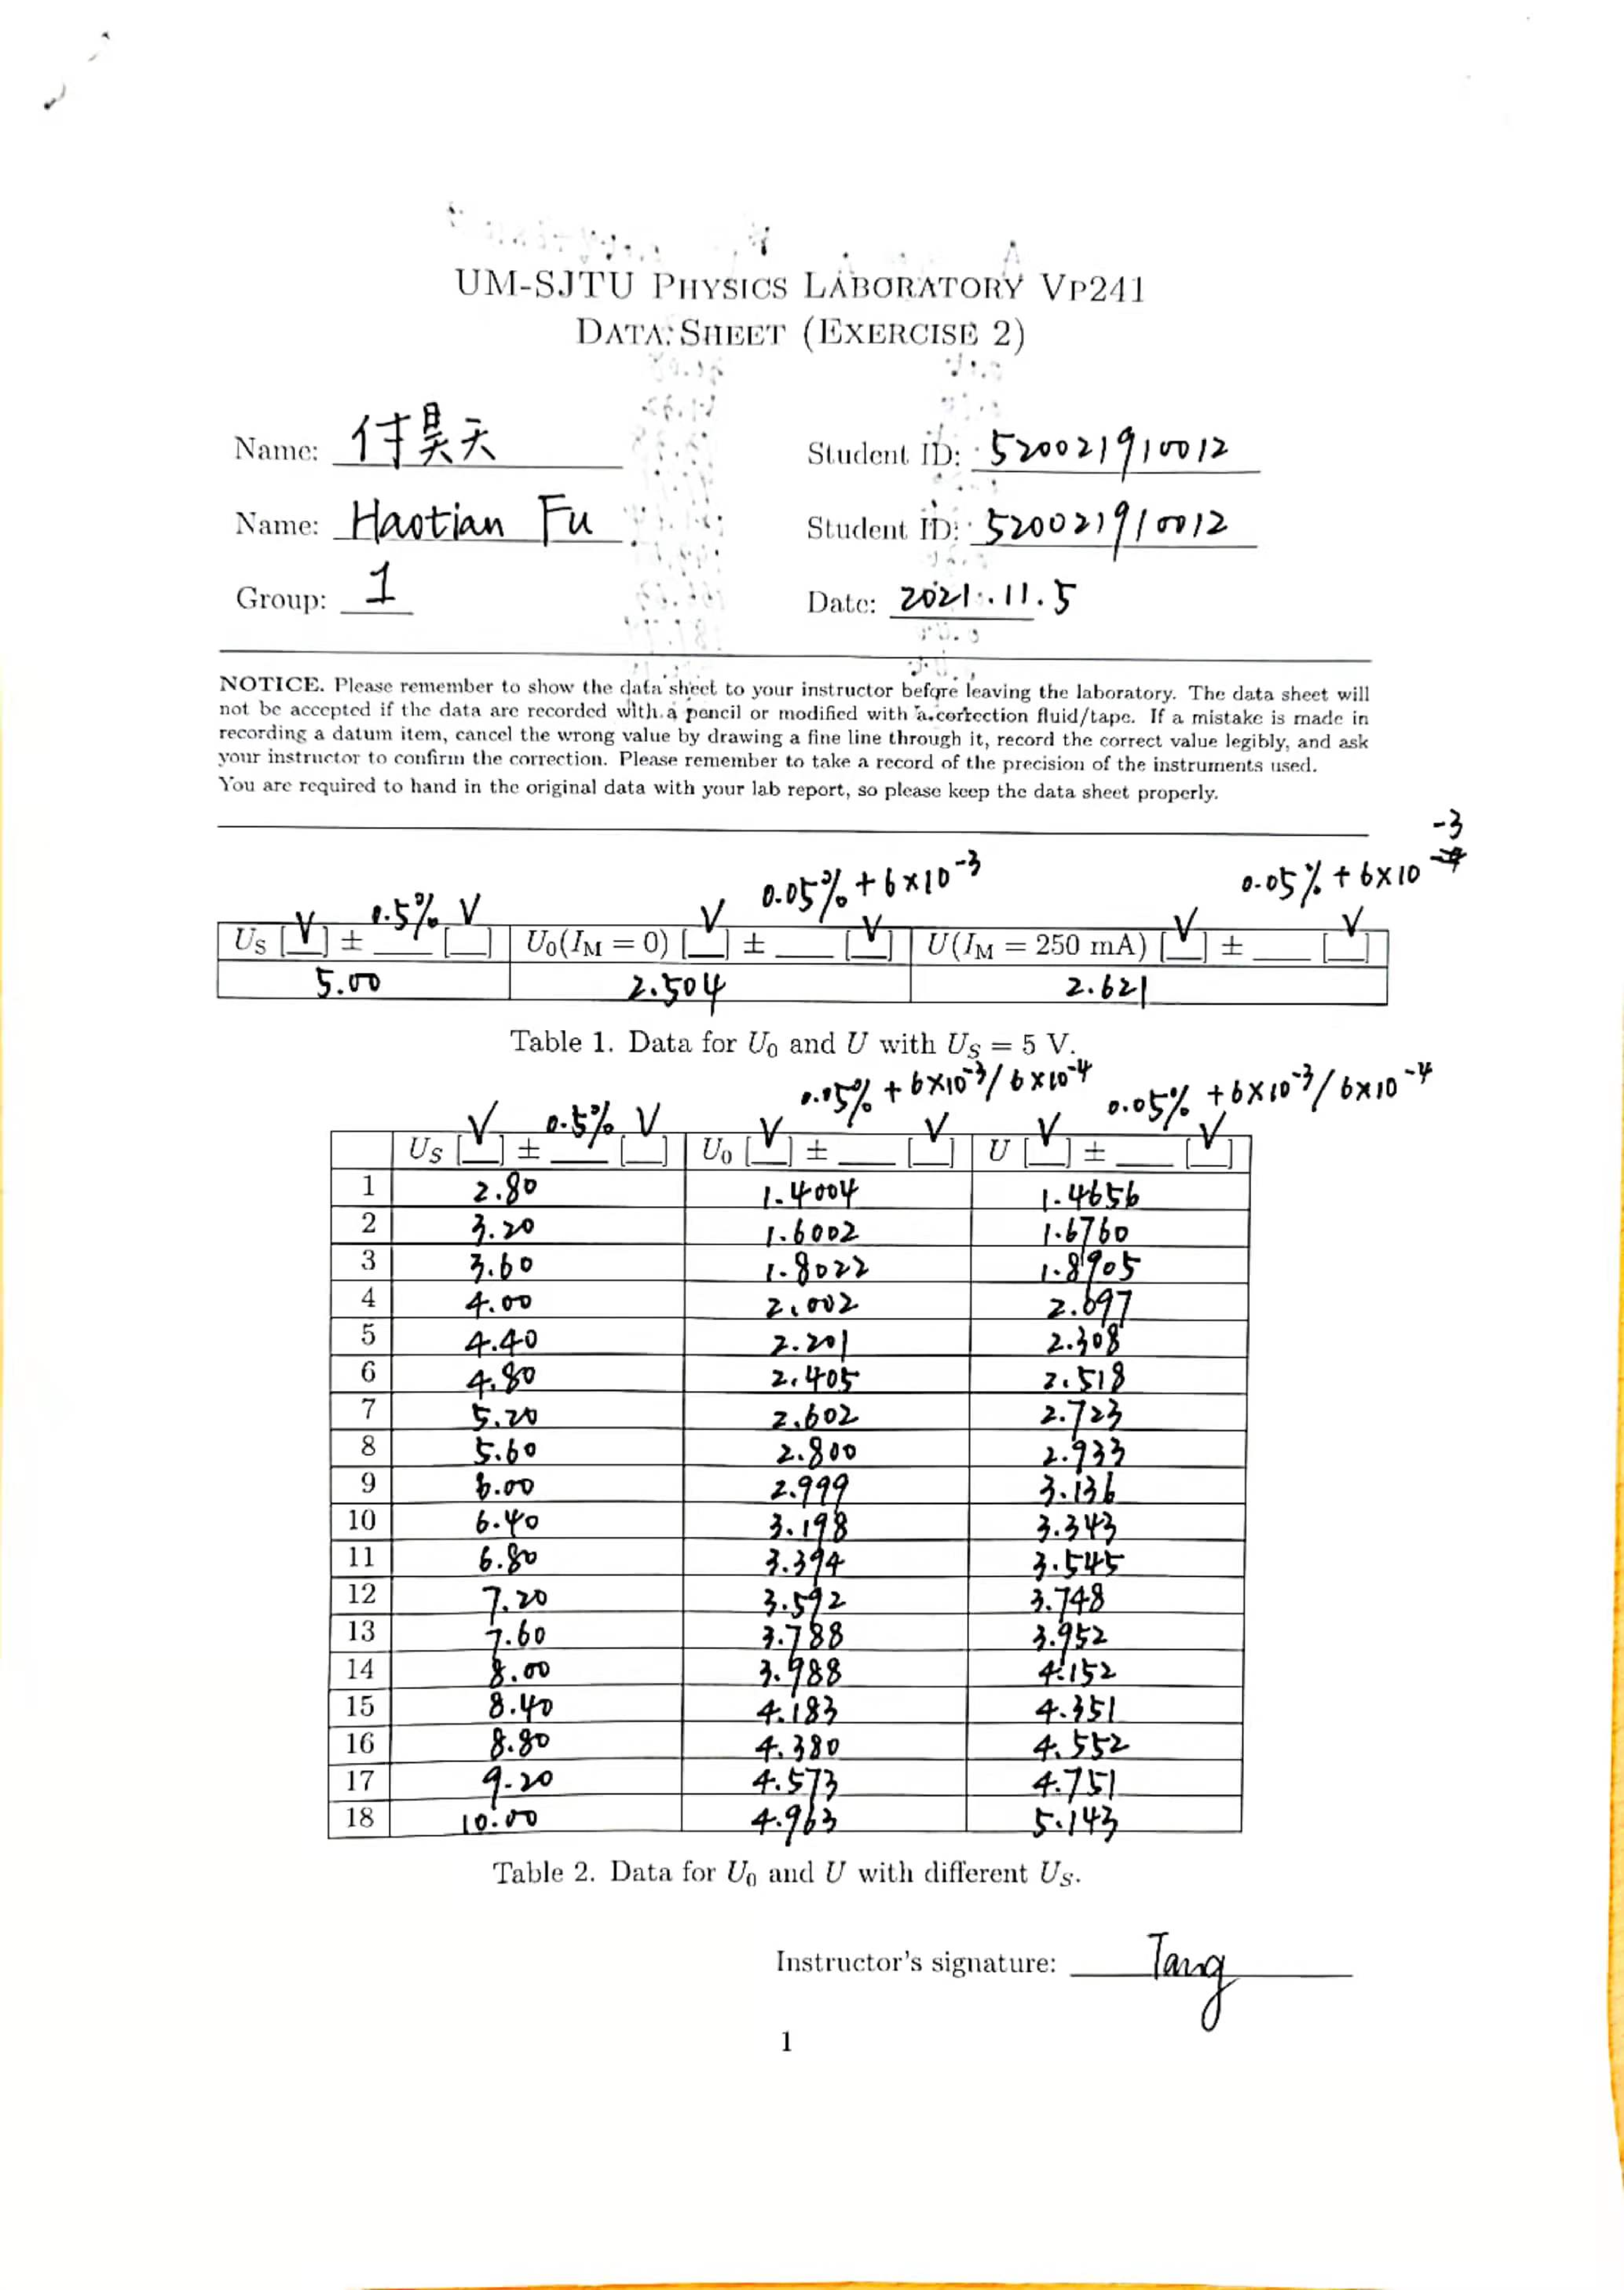
\includepdf{data_sheet_1.pdf}
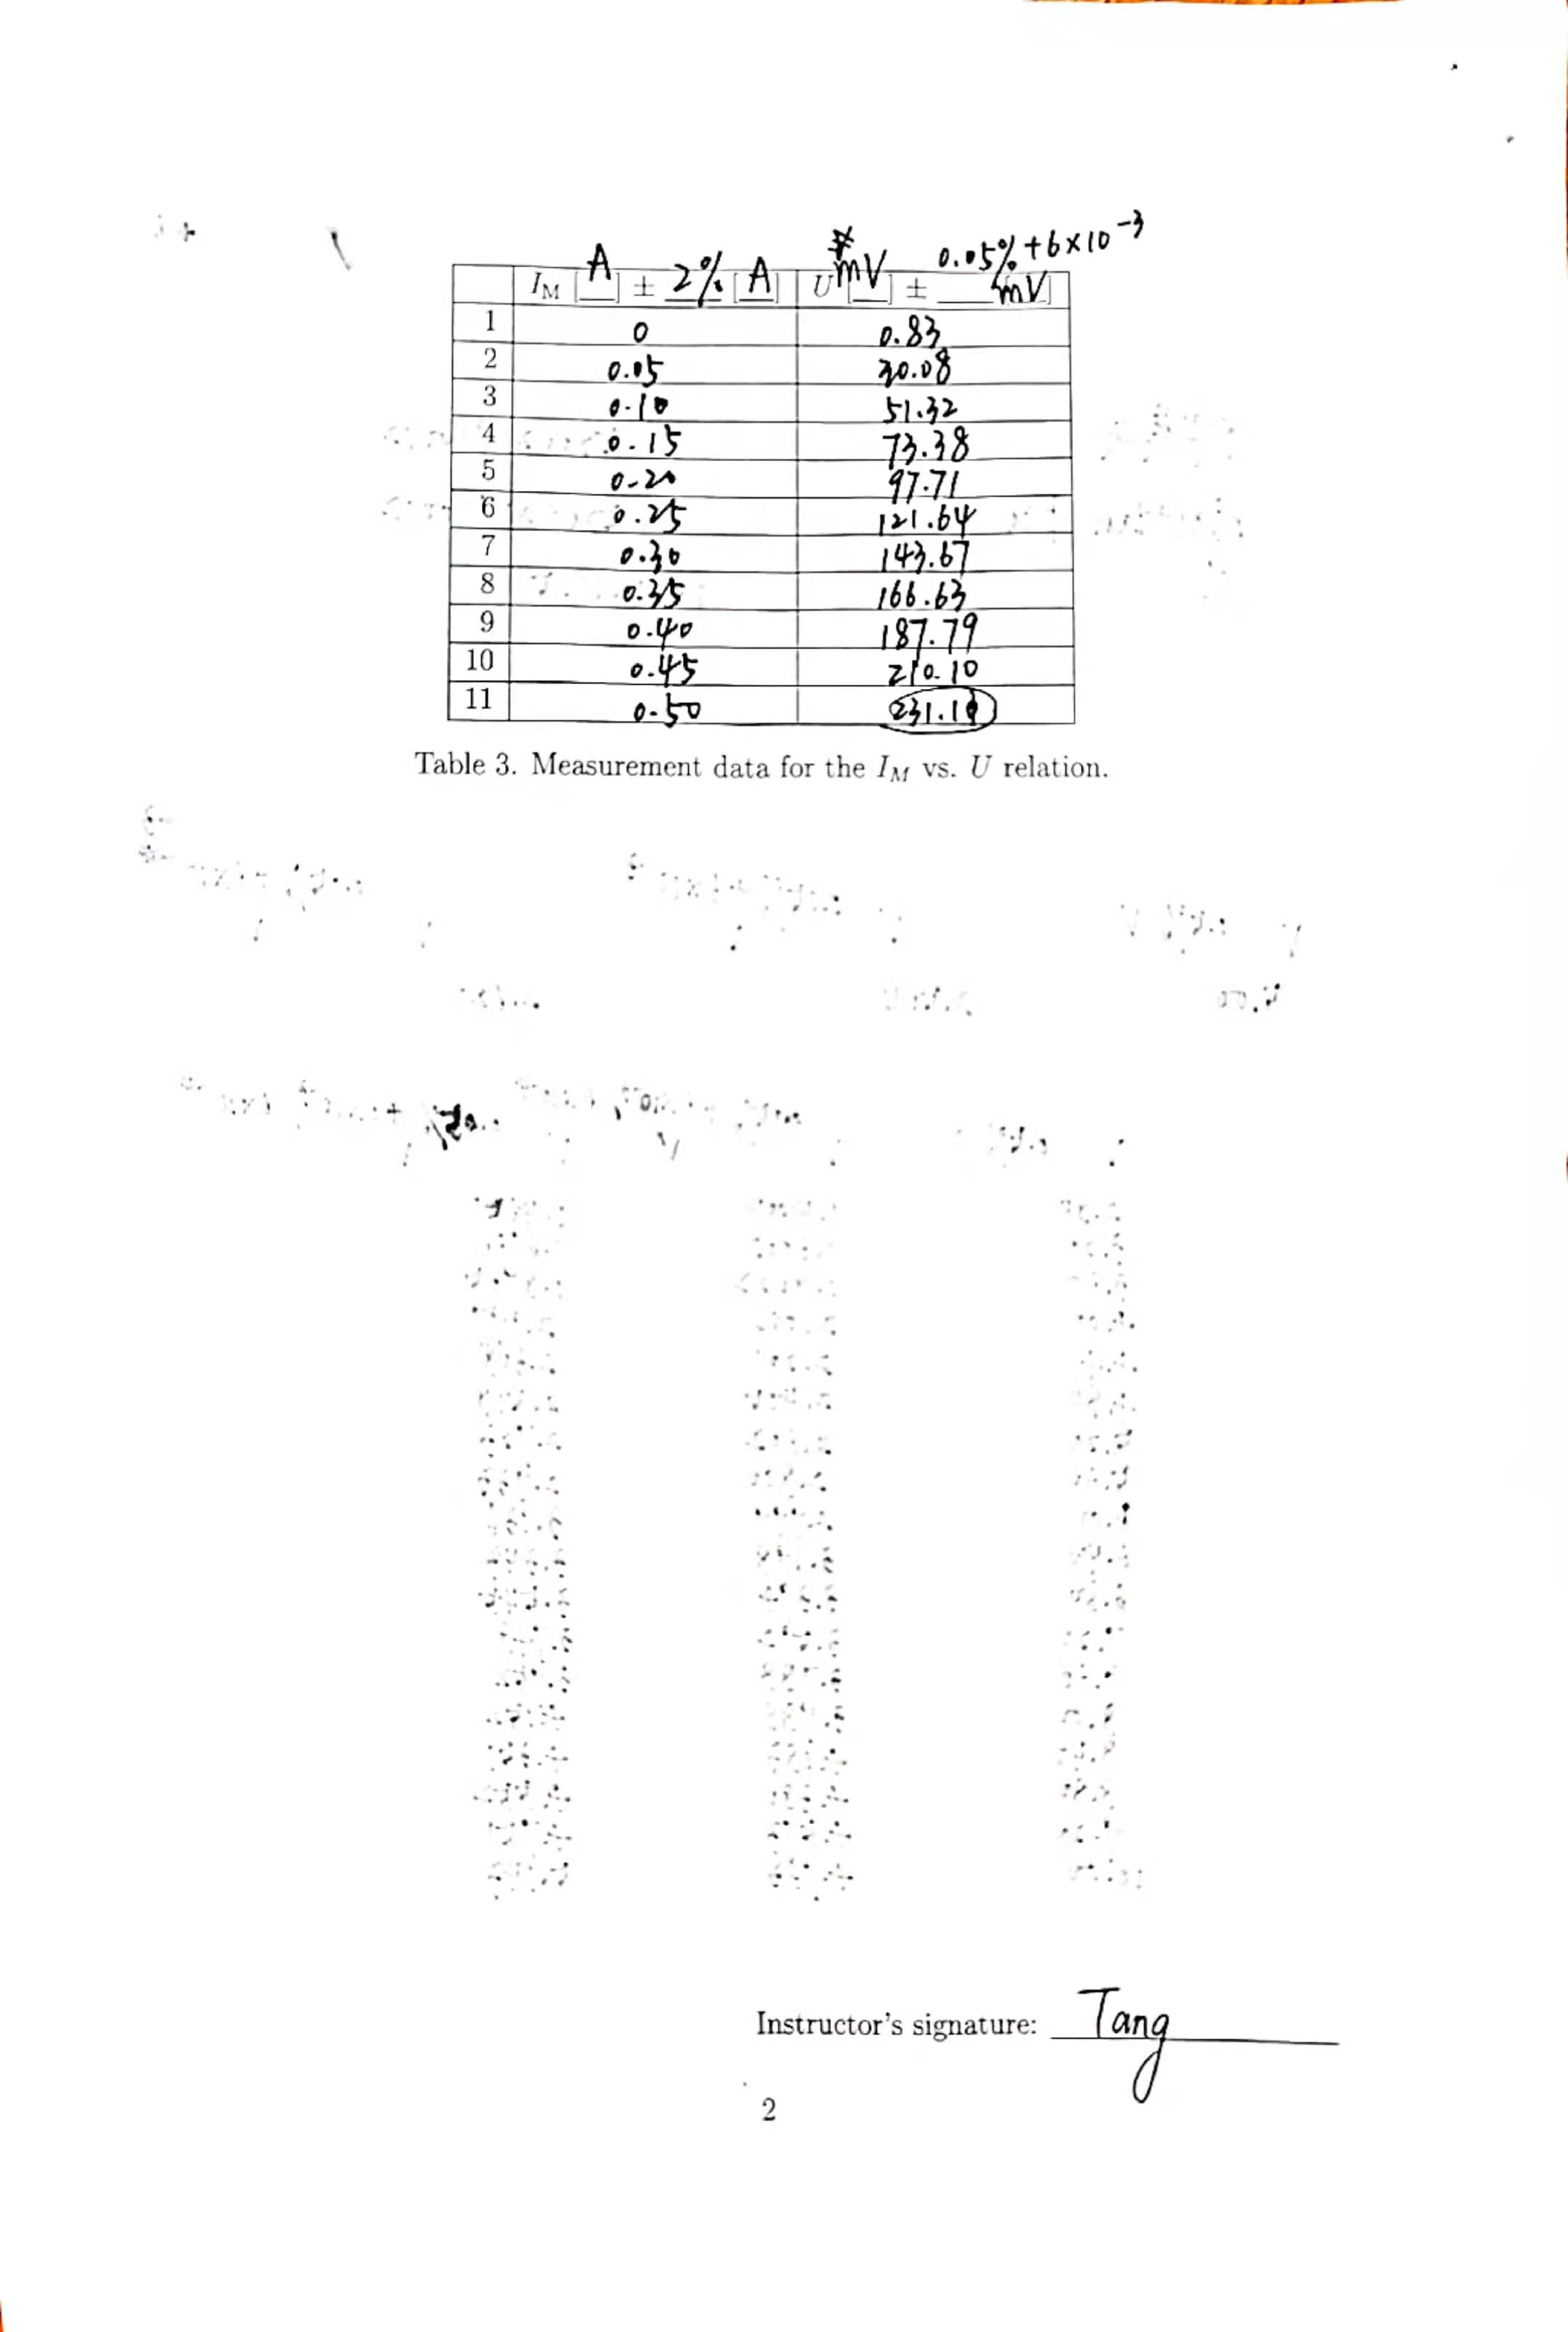
\includepdf{data_sheet_2.pdf}
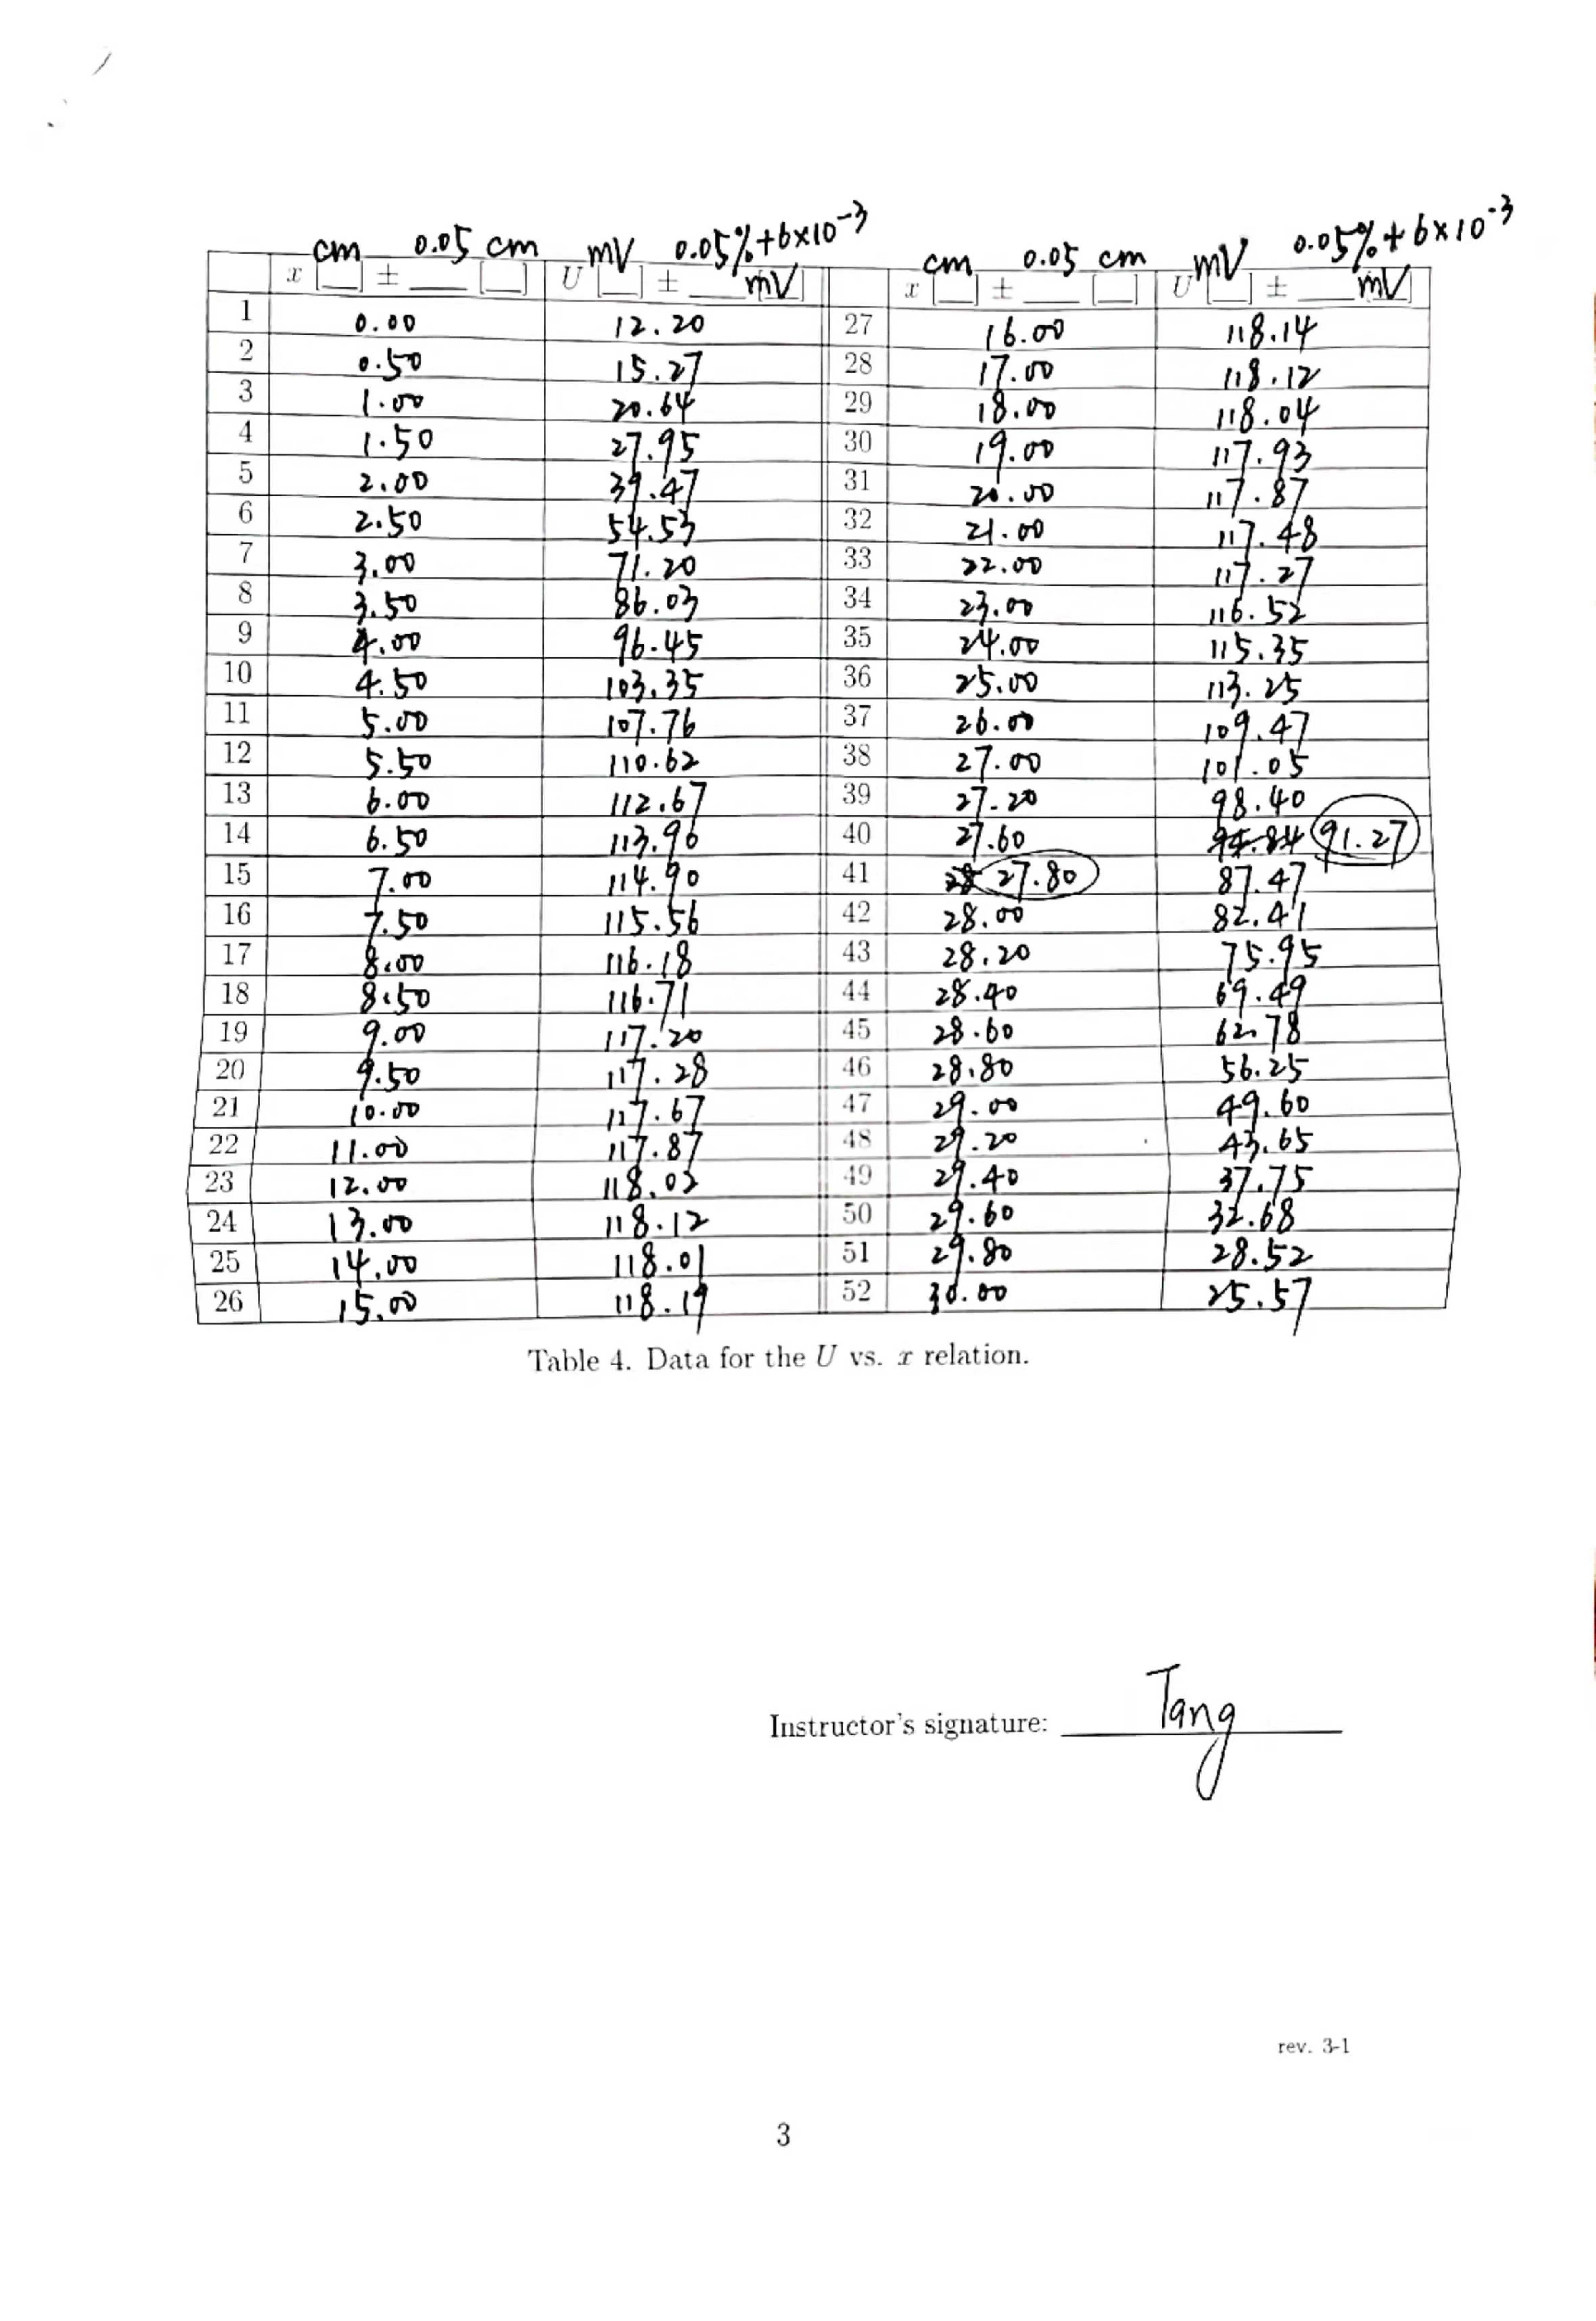
\includepdf{data_sheet_3.pdf}

\end{document}
